%CLASSE DOCUMENTO - LINGUA E DIMENSIONE FONT
\documentclass[corpo=11pt,numerazioneromana]{toptesi}

%%%%%%%%%%%%%%%%%%%%%%%%%%%%%%%%%%%%%%%%%%%%%%%%%%%%%%%%%%%%%%%
\usepackage[top=3cm,bottom=3cm,left=4cm,right=2.5cm,headsep=10pt,letterpaper]{geometry} % Page margins
% INCLUSIONE PACCHETTI
\usepackage[classica]{topfront}
\usepackage[utf8]{inputenc} %utf8
\usepackage[italian]{babel}
\usepackage[T1]{fontenc}
\usepackage{blindtext}
\usepackage{graphicx,wrapfig}
\usepackage{booktabs}
\usepackage{lmodern}
\usepackage{varioref}
\usepackage{url}
\usepackage{array}
\usepackage{paralist}{\obeyspaces\global\let =\space}
\usepackage{verbatim}
\usepackage{subfig}
\usepackage{tabularx}
\usepackage{amsmath}
\usepackage{amsfonts}
\usepackage{pdfpages}
\usepackage{float}
\usepackage{amssymb}
\usepackage{multicol}
\usepackage{multirow}
\usepackage{afterpage}
\usepackage{listings}
\usepackage[figuresright]{rotating}
\usepackage{algorithm}
\usepackage{algorithmic}
\usepackage{amsmath}
\usepackage[babel]{csquotes}
\usepackage{hyperref}
\usepackage[backend=biber,bibencoding=ascii]{biblatex}

\newcommand\blankpage{%
    \null
    \thispagestyle{empty}%
    \addtocounter{page}{-1}%
    \newpage}
\makeatletter
\newcommand\listofcodes{%
 \iffrontmatter\else\frontmattertrue\fi
 \if@openright\cleardoublepage\else\clearpage\fi
 % change the meaning of \chapter in a group
 \begingroup\def\chapter##1{\@schapter}
 \phantomsection % for the hyperlink
 \addcontentsline{toc}{chapter}{Elenco dei codici}
 \lstlistoflistings
 \endgroup
} 
\makeatother

\addto\captionsitalian{%
  \renewcommand{\lstlistlistingname}{Elenco dei codici}%
  \renewcommand{\lstlistingname}{Codice}%
}
%%%%%%%%%%%%%%%%%%%%%%%%%%%%%%%%%%%%%%%%%%%%%%%%%%%%%%%%%%%%%%%

% CONFIGURAZIONE LINK E RIFERIMENTI
\hypersetup{%
    pdfpagemode={UseOutlines},
    bookmarksopen,
    pdfstartview={FitH},
    colorlinks,
    linkcolor={black}, %COLORE DEI RIFERIMENTI AL TESTO
    citecolor={blue}, %COLORE DEI RIFERIMENTI ALLE CITAZIONI
    urlcolor={blue} %COLORI DEGLI URL
}

%%%%%%%%%%%%%%%%%%%%%%%%%%%%%%%%%%%%%%%%%%%%%%%%%%%%%%%%%%%%%%%

% CONFIGURAZIONE LISTATI/CODICE - CANCELLARE SE NON NECESSARIO
% PYTHON - BIANCO E NERO
\lstset{%
	captionpos=b,
	language=Python,
	basicstyle =\small\ttfamily,
	keywordstyle=\color{black}\bfseries,
	breaklines=true,
	breakatwhitespace=true,
	frame=lines,
	numbers=left,
	numberstyle=\footnotesize,
}

%%%%%%%%%%%%%%%%%%%%%%%%%%%%%%%%%%%%%%%%%%%%%%%%%%%%%%%%%%%%%%%

% FRENCHSPACING VA _SEMPRE_ ABILITATO PER DOCUMENTI IN ITALIANO
\frenchspacing

%%%%%%%%%%%%%%%%%%%%%%%%%%%%%%%%%%%%%%%%%%%%%%%%%%%%%%%%%%%%%%%

%%%%%%%%%%%%%%%%%%%%%%%%%%%%%%%%%%%%%%%%%%%%%%%%%%%%%%%%%%%%%%%

\hypersetup{
    pdfauthor={Claudio Di Salvo},
    pdfsubject={Tesi Triennale in Ingegneria elettronica ed informatica},
    pdftitle={Implementazione di meccanismi per la Full e PartialReconfiguration di FPGA in architetture IoT-Cloud},
    pdfkeywords={FPGA, Full reconfiguration, Partial Reconfiguration}
}

%%%%%%%%%%%%%%%%%%%%%%%%%%%%%%%%%%%%%%%%%%%%%%%%%%%%%%%%%%%%%%%

% LISTA DEI CAPITOLI DA INCLUDERE - PERSONALIZZARE
\includeonly{%
Introduzione,%
Background,%
Capitolo1,%
Capitolo2,%
Capitolo3,%
Capitolo4,%
Capitolo5,%
Conclusioni,%
app_a,%
}

% FILE DI BIBLIOGRAFIA
\addbibresource{bibliography.bib}

%%%%%%%%%%%%%%%%%%%%%%%%%%%%%%%%%%%%%%%%%%%%%%%%%%%%%%%%%%%%%%%

% INIZIO DOCUMENTO
\begin{document}



\includepdf{frontespizio.pdf}
\afterpage{\blankpage}
%%%%%%%%%%%%%%%%%%%%%%%%%%%%%%%%%%%%%%%%%%%%%%%%%%%%%%%%%%%%%%%

%INTERLINEA - DEFAULT 1 - NON ESAGERATE, NON SUPERATE MAI 1.3 ;)
\interlinea{1.5}

%%%%%%%%%%%%%%%%%%%%%%%%%%%%%%%%%%%%%%%%%%%%%%%%%%%%%%%%%%%%%%%

\frontmatter


%%%%%%%%%%%%%%%%%%%%%%%%%%%%%%%%%%%%%%%%%%%%%%%%%%%%%%%%%%%%%%%

% INDICI - ELIMINARE GLI INDICI NON NECESSARI

% INDICE GENERALE
\tableofcontents

% INDICE DELLE FIGURE
\listoffigures

\listofcodes




%%%%%%%%%%%%%%%%%%%%%%%%%%%%%%%%%%%%%%%%%%%%%%%%%%%%%%%%%%%%%%%

\mainmatter
% INCLUSIONE FILE CAPITOLI - PERSONALIZZARE - TENERE COERENTE CON LISTA IN ALTO
\chapter{Introduzione}
\label{chap:intro}


\chapter{Background}
\label{chap:background}
Al fine di fornire le conoscenze necessarie alla comprensione od eventuale continuazione del lavoro svolto in questo elaborato, risulta necessario introdurre gli argomenti che si andranno ad affrontare durante la tesi, partendo dai dispositivi FPGA.
\section{Field Programmable Gate Array}
\label{FPGA}
Sin dal invenzione dei computer, la loro progrettazione è avvenuta con una rapida evoluzione. A metà degli anni '80, un tipo di architettura diverso da quello convenzionale fu sviluppato, le Field Programmable Gate Array (FPGA). Esse furono costruite tramite un interconnessione effettuata dal progettista tra ROM/PROM o array di porte NAND.
Le FPGA moderne, sono una soluzione prefabbricata, elettronicamente programmabile, atte alla progettazione di sistemi digitali ad alte prestazioni per basso volume. Le FPGA vengono progettate su CAD appositi, come ad esempio VIVADO, senza la necessità di dover modificare la struttura fisicamente.\clearpage
\begin{figure}[h]
\centering
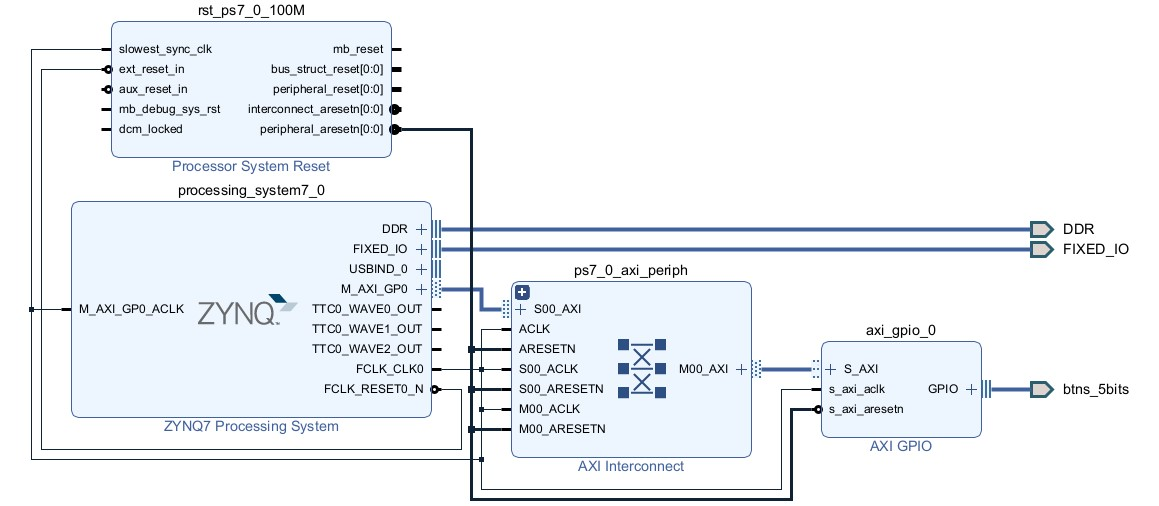
\includegraphics[width=0.8\textwidth]{images/Vivado.jpg}
\caption{Foto di una prototipazione tramite vivado di una FPGA zynq-7000 che sfrutta il GPIO}
\label{VIVADO1}
\end{figure}
Questa famiglia di dispositivi dev'essere immaginataa come un insieme di componenti logici, tali Configurable Logic Block (CLB), come già detto possono essser modificati dal progettista, i CLB sono composti da Look Up Table (LUT), Full Adders, Registi, Multiplexer e funzioni date dall'implementazioni.
Questa divisione in blocchi permette di creare dei cluster interconnessi, rendendo cosi possibile la sintetizzazione di tutte le possibili operazioni booleane e la realizzazione di sistemi complessi. 
\begin{figure}[h]
\centering
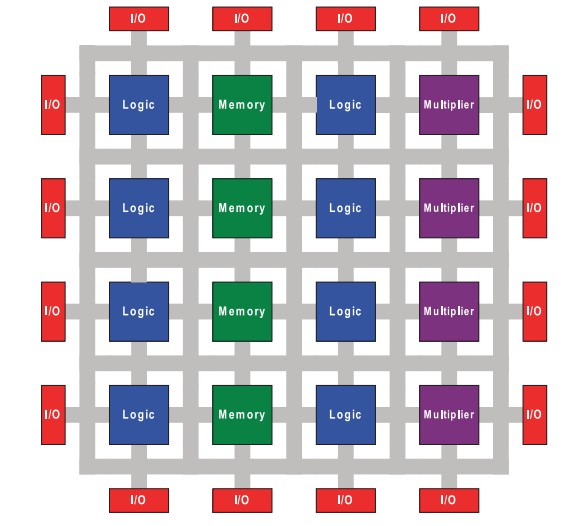
\includegraphics[width=0.3\textwidth]{images/FPGA.jpg}
\caption{Tipica rappresentazione di un FPGA \cite{8187326}}
\end{figure}\\
Le FPGA per loro natura devono comunicare in qualche modo con altri dispositivi, tale comunicazione è gestita da blocchi detti Input Output Block(IOB), essi garantiscono l'interfacciamento tra le risorse della programmable logic (PL) ed il mondo esterno, ogni IOB gestisce un segnale d'input/output ed è in grado di effettuare una conversione, programmabile, tra formati seriali e paralleli, oltre alla gestione di vari standard di I/O e l'eventuale configurazione di Pull-up/Pull-down interni.\\
Data la sempre più crescente quantità di CLB si può pensare come sia necessario aumentare sempre di più l'area di silicio occupata, ma essa è solitamente occupata dai sistemi di interconnessione interna.\\
Le FPGA essendo completamente riprogrammabili possono accogliere dei cores custom, detti Intellectual Property Cores, essi rappresentano dei dispositivi pre-realizzati al fine di compiere una ben precisa azione, essi possono passare da un banale moltiplicatore ad un softcore arm.
\begin{figure}[h]
\centering
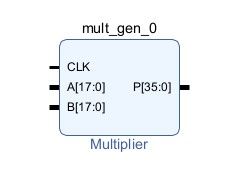
\includegraphics[width=0.3\textwidth]{images/IPcores.jpg}
\caption{Rappresentazione grafica di un IPCore in Vivado}
\end{figure}\\
\subsection{Le FPGA SoC}
L'evoluzione dei processi tecnologici ha portato alla nascita di nuovi tipi di FPGA, le FPGA SoC, esse sono architetture che presentano una interconnessione tra Processore, solitamente della famiglia ARM, ed un FPGA in un unico dispositivo.\clearpage
\begin{figure}[h]
\centering
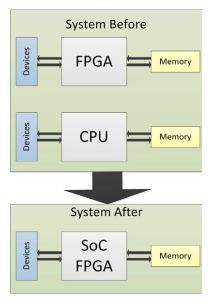
\includegraphics[width=0.4\textwidth]{images/Capture1.png}
\caption{Cambio di paradigma con l'introduzione delle FPGA SoC}
\end{figure}
La loro fusione permette una maggior integrazione, anche lato connettività e quindi Cloud, un minor consumo ed una comunicazione molto più efficiente tra i due grazie ad una larghezza di banda superiore ed una latenza nettamente inferiore a prima.
\begin{figure}[h]
\centering
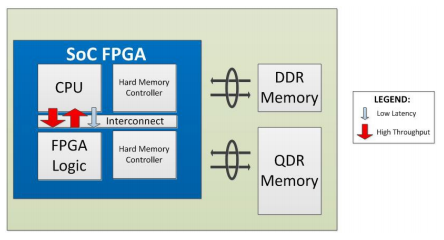
\includegraphics[width=0.6\textwidth]{images/Capture8.png}
\caption{Schema rappresentativo FPGA SoC}
\end{figure}\\
\subsection{Architettura Zynq-7000}
L'architettura Zynq-7000 è basata sul architettura Xilinx All Programmable System On Chip (AP SoC). I dispositivi di questa famiglia sono formati da un dual-single Core ARM Cortex A9 su cui si basa il Processing System (PS), includendo anche una on-chip memory, interfacce con memorie esterne e le periferiche di connettività con le interfacce, ed una Programmable Logic (PL) a 28nm.\\
La PS e la PL sono alimentate separatamente e sarà compito del progettista decidere se disabilitare o meno la Programmable Logic, il processore eseguira il boot per primo e sarà sempre necessario anche per usare la parte logica, infatti si usa un approccio software centrico per la PL, ma come vedremo più avanti le due parti non sono scollegate tra di loro e questo approccio ci servirà al fine di effettuare operazioni lato PL.
\begin{figure}[h]
\centering
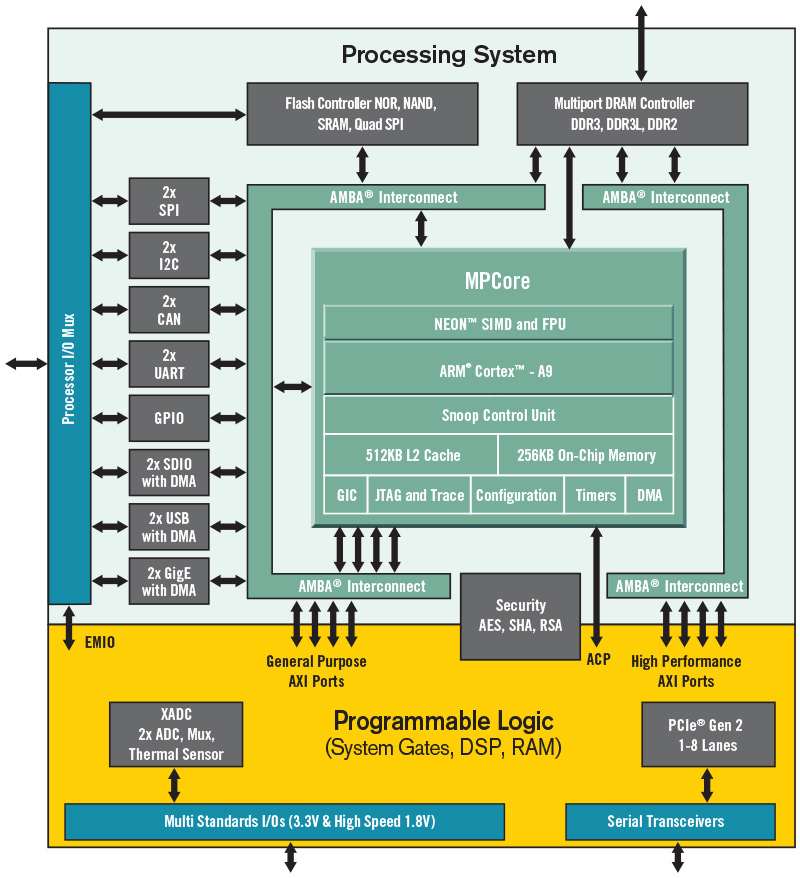
\includegraphics[width=0.6\textwidth]{images/zynq_arch.png}
\caption{Schema rappresentativo ZYNQ-7000\cite{Zynq-7000}}
\end{figure}\\
\section{Linguaggi di descrizione delle FPGA}
Come accennato nel capitolo, \ref{FPGA}, le FPGA vengono implementate tramite l'uso dei CAD da un progettista, risulta però utile avere conoscenze dei linguaggi di descrizione dell'hardware quali VHDL\cite{VHDL} e Verilog\cite{Verilog} . Entrambe le opzioni sono supportate da Vivado e sono valide al fine di descrivere il comporamento di un sistema digitale. Le principali differenze tra i due linguaggi sono le similitudini al linguaggio C, infatti il Verilog ricorda molto la struttura del linguaggio di programmazione, permettendo anche ad un utente novizio la comprensione e l'appoccio a questo tipo di linguaggio.\\
In generale entrambi i linguaggi sono intercambiabili per quanto rigurda la rappresentazione Register Transfer Level, ovvero la schematizzazione del sistema come un flusso di informazioni tra logica e registri. Inoltre entrambi condividono una struttura gerarchica, infatti è possibile tramite dei costrutti descrivere un sistema in maniera strutturale, tramite tre possibili approcci:
\begin{itemize}
    \item Comportamentale: Il programmatore ha il compito di descrivere il comportamento di un sistema tramite un algoritmo.
    \item Strutturale: Il programmatore descrive singolarmente ogni componente interno al sistema andando poi ad usare una combinazione per rappresentare il sistema.
    \item DataFlow: Il programmatore scrive il codice emulando il flusso di dati nel sistema.
\end{itemize}
Ogni approccio necessità la presenza di un Top Level Entity, ovvere il file principale che verrà sintetizzato e che ci permetterà di implementare l'FPGA, esso conterrà tutte le componenti, codici ed eventuali librerie o supporti.
\begin{figure}[h]
\centering
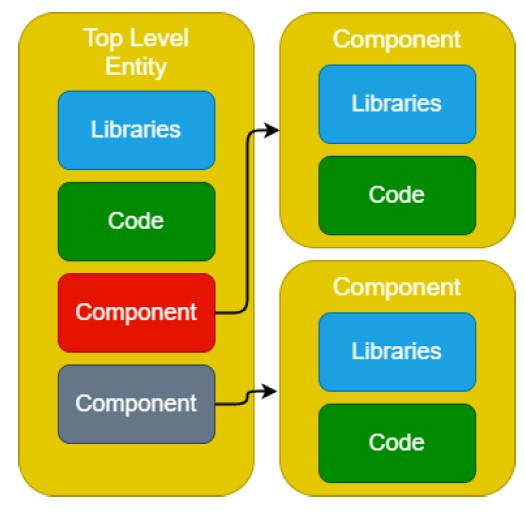
\includegraphics[width=0.3\textwidth]{images/VHFL.jpg}
\caption{Rappresentazione grafica di una Top Level Entity\cite{TesiMattia}}
\end{figure}\\
Una volta terminata la stesura del codice, ad oggi si usa solitamente per la creazione di IPCores custom, bisogna specificare le specifiche e limitazioni, i \textit{constraints}, che sono necessarie affinchè il sistema possa esser realizzato sulla scheda.
\section{Processo di Sviluppo FPGA}
Il processo di sviluppo non è riducibile alla scrittura del codice di definizione, come potrebbe avvenire per un arduino, ma necessità dei passaggi ulteriori dovuti all'architettura, infatti la presenza dell'interconnessione dei blocchi, i blocchi I/O necessariamente configurati e la programmable logic definita necessità la presenza di passaggi ulteriori.\\
L'evoluzione tecnologica ha portato ad avere grosse migliorie per quanto riguarda lo sviluppo, infatti ad oggi si parte dalla scrittura del codice\footnote{O generazione di esso tramite vivado}, passando il tutto ad un sistema di sintesi che ci permette di tradurre il tutto in una netlist, esso è un file che ci descrive tutte le interconnessioni logiche da effettuare tra i vari blocchi della scheda.\\

Per capire meglio il funzionamento dividiamo il processo in tre stadi:
Il primo stadio che prende il nome di \textit{Technology Mapping},effettua la generazione di un modello RTL (Register Transfer Level), questo stadio converte il codice di descrizione in dei blocchi più semplici, è importantissimo poichè bisogna garantire che le funzionalità descritte nel codice siano rispettate, esso si verifica tramite delle simulazioni. Alcuni blocchi di logica complessa vengono portati ad un livello composto tra gate logici e registri questo livello è detto Logic Gate Level.
\begin{figure}[h]
\centering
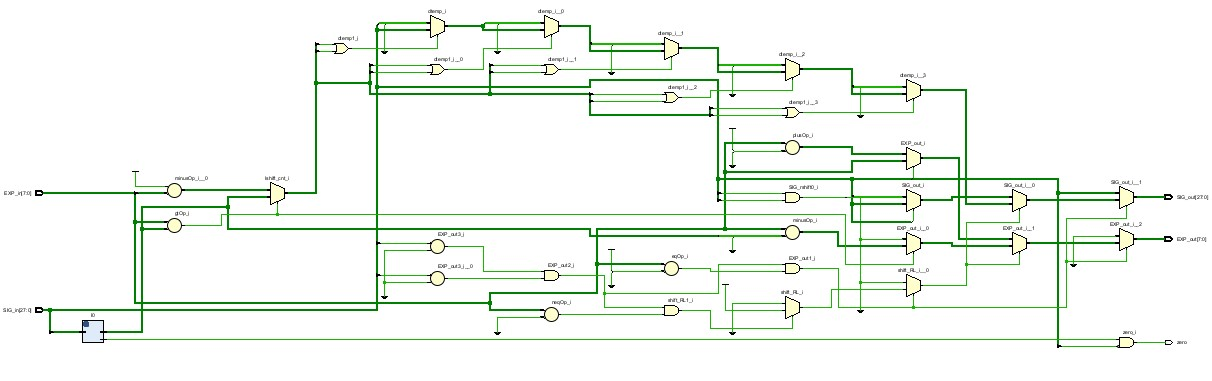
\includegraphics[width=0.8\textwidth]{images/RTL.jpg}
\caption{Rappresentazione grafica del Tecnology Mapping del FPGA in figura \ref{VIVADO1}}
\end{figure}\clearpage
Tutto questo processo viene ottimizzato come farebbe un compilatore, al fine di occupare meno spazio.\\
Una volta effettuato questo passaggio bisogna effettuare la collocazione degli elementi dell'FPGA, il procedimento prende il nome di \textit{Place \& Route} (\textit{PnR}), esso a sua volta è composto da tre sotto passaggi.\\
Il primo è il \textit{Packing}, esso analizza le primitive e le organizza in un cluster.\\
Il secondo è il \textit{Placing} prende in ingresso i cluster ed effettua la decisione di dove piazzare fisicamente i componenti sulla scheda permettendo cosi l'instradamento
\begin{figure}[h]
\centering
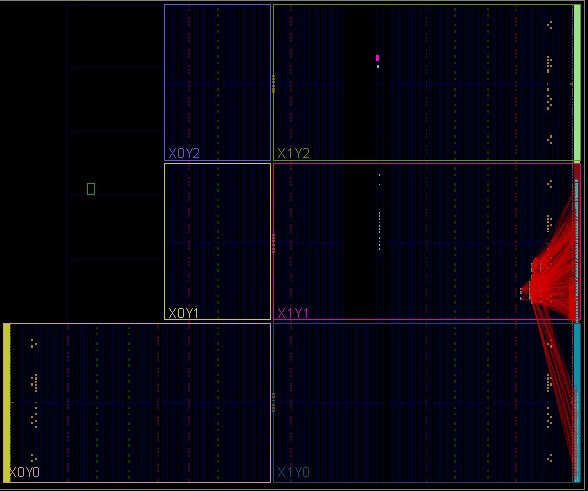
\includegraphics[width=0.4\textwidth]{images/Place.jpg}
\caption{Rappresentazione grafica del Placing del FPGA in figura \ref{VIVADO1}}
\end{figure}\\
In fine il \textit{Routing}, si occuperà di calcolare tutte le possibili connessioni scegliendo la migliore, in funzione del ritardo questo ovviamente rende il passaggio oneroso computazionalmente.
\begin{figure}[h]
\centering
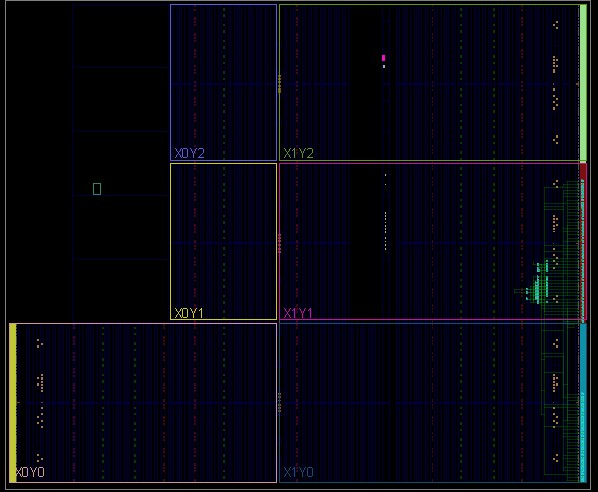
\includegraphics[width=0.4\textwidth]{images/Route.jpg}
\caption{Rappresentazione grafica del Routing del FPGA in figura \ref{VIVADO1}}
\end{figure}\\
Una volta terminati questi passaggi avremo a disposizione l'implementazione del FPGA, ma sarà necessario tradurre il tutto in un formato interpretabile al dispositivo, questo processo verrà ripreso anche in seguito. Questo passaggio di traduzione prende il nome di generazione del bitstream.
\begin{figure}[h]
\centering
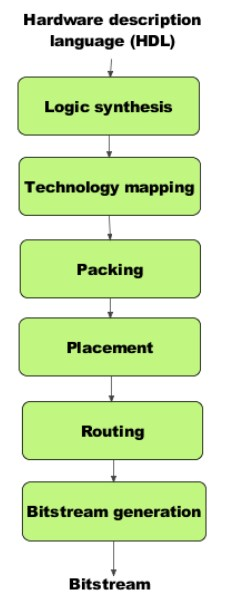
\includegraphics[width=0.2\textwidth]{images/Stack.jpg}
\caption{Stack per lo sviluppo di un FPGA}
\end{figure}\\
Questo tipo di sviluppo è il migliore nel nostro caso poichè non stiamo effettuando un High Level Synthesis (HLS), in quel caso esistono dei tools appositi.
\subsection{Sviluppo tramite Vivado}
Lo sviluppo tramite vivado è al quanto semplificato, poichè godendo di un interfaccia grafica permette l'implementazione di sistemi complessi anche non avendo alcuna conoscenza di VHDL o Verilog, si rimanda però all'appendice \ref{app:a} per maggiori chiarimenti su installazione ed inizio del primo progetto.
\section{Tecnologie implementative}
\subsection{Vitis}
Vitis è il Software Development Kit (SDK) fornito da Xilnix nella sua suite di prodotti, la sua installazione è contestuale a quella trattata in \ref{app:a}, tramite esso è possibile generare codice che in grado di esser eseguito sulla scheda, questo è possibile tramite le informazioni prese su vivado.\\
Sono presenti due possibilità di programmazione, standalone e linux, la prima applicazione permetterà l'esecuzione di codice C in modalità Bare-Metal\footnote{Livello di programmazione senza astrazioni, come il sistema operativo}, in questo modo potremmo usare delle librerie della Xilinix che contengono delle funzioni standard al fine di effettuare la comunicazione tra PS e PL. Successivamente tratteremo anche la comunicazione tra PS e PL su sistema linux. Questo tipo di programmazione è discussa approfonditamente \ref{Standalone}
\subsection{Petalinux}
È un tool della Xilinix che necessario qualora si volesse usare una distro Linux embedded su di una FPGA SoC xilinix, la sua installazione è trattata in \ref{petalinuxinst}. Petalinux offre una grossa flessibilità per la costruzione e compilazione di un kernel Linux, la sua flessibilità ci permette di escludere o includere moduli pre-esistenti oppure crearne uno noi secondo le nostre esigenze. Si basa fortemente sull'architettura e sull'esportazione che avviene da vivado al fine di costruire il device tree e tutti gli strumenti necessari al kernel.\\
Al fine di usufruire di petalinux vanno impostati i Jumpers della scheda MIO2-6 in configurazione  "00110", in questo modo potremmo usare il kernel che abbiamo creato e compilato\footnote{Che vedremo successivamente}, tramite la scheda SD che dovrà rispettare delle specifiche espresse in \ref{sd}.
\subsection{Bootgen}
\textit{Bootgen} è un tool appartenente alla suite di sviluppo della Xilinix, il suo scopo è quello di generare i file binari e tutti gli artefatti necessari. La sua installazione verrà discussa in \ref{installazioneBoot}
Sfortunatamente questo tool è attualemente disponibile solo per architettura x86, quindi come tutti i tool presentati precedentemente non sarà possibile installarli sulla piattaforma da noi prescelta.\clearpage
\subsection{OpenStack}
OpenStack è un piattaforma cloud open-source\cite{OpenStack2} che permette la gestione di risorse in cloud, queste risorse possono variare da macchine virtuali, blocchi d'indirizzamento, spazio d'archiviazione ed acceleratori. Tutte le risorse fisiche vengono aggregate in un unico grande pool ed alloca le risorse virtuali permettendo cosi la richiesta tramite le API da parte dell'utente finale, OpenStack non gestisce la virtualizzazione, ma sfrutta le tecnologie di virtualizzazioni preesistenti eseguendo un funzionamento assimilabile a quello di un raccoglitore.
\begin{figure}[h]
\centering
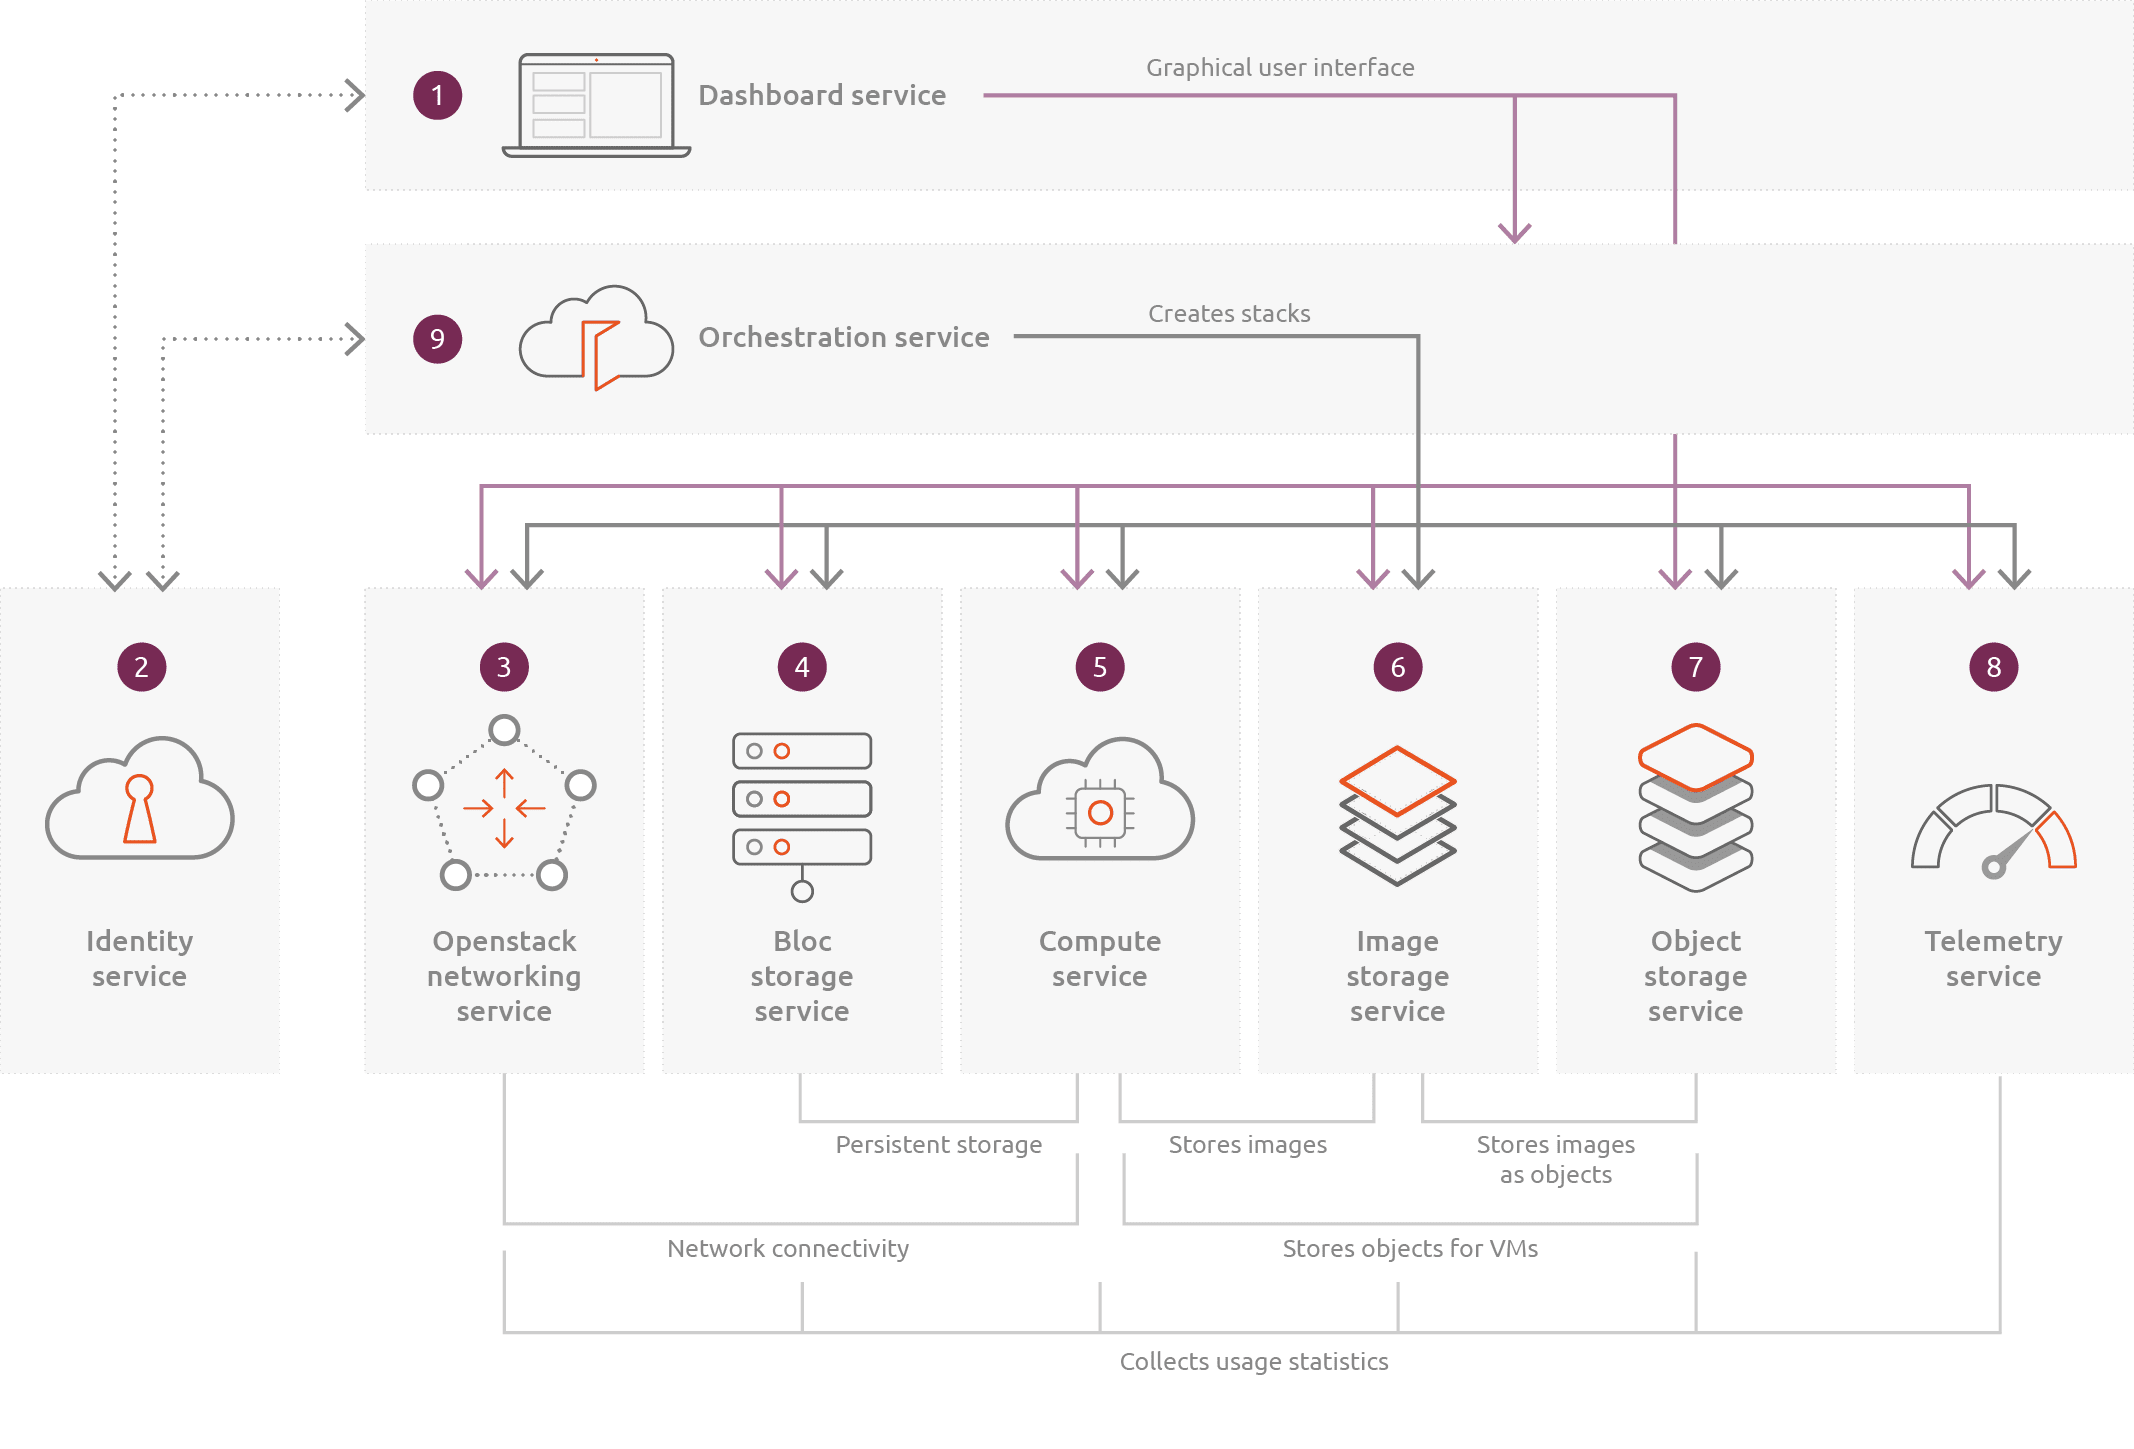
\includegraphics[width=1\textwidth]{images/Openstack.jpg}
\caption{Diagramma rappresentativo funzionamento OpenStack\cite{OpenStack2}}
\end{figure}\\
\subsection{Nova}
Nova fa parte del progetto open-source OpenStack, il suo scopo è la gestione delle Virtual Machine (VM), esso permette, in simbiosi con Cyborg, di definire gli acceleratori e le FPGA come VM, per maggiori approfondimenti si rimanda a \cite{Nova}.
\subsection{Cyborg}
È un sottosistema di OpenStack, il quale si occupa della gestione del ciclo di vita degli acceleratori, il tutto viene effettuato tramite un interfaccia \textit{REpresentational State Transfer} (REST), tale approccio permette l'aggiunta e la rimozione di nodi ed informazioni legate ai dispositivi.\cite{Cyborg}
\begin{figure}[h]
\centering
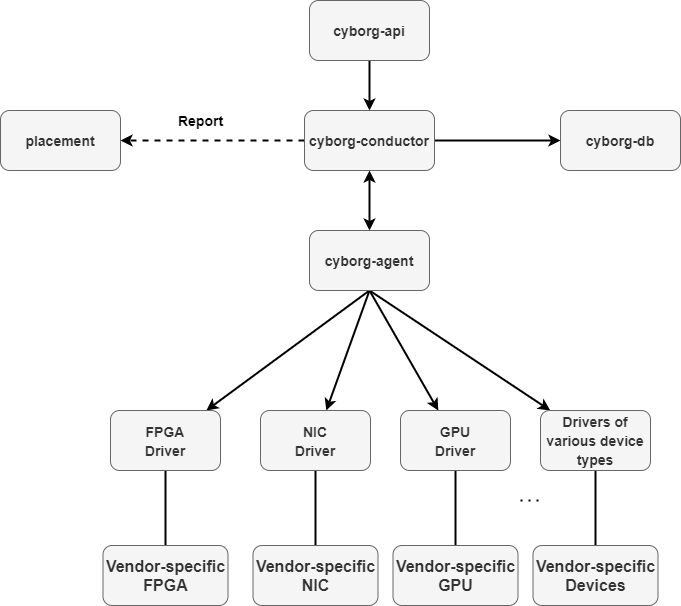
\includegraphics[width=0.7\textwidth]{images/cyborg-architecture.png}
\caption{Architettura del funzionamento di Cyborg\cite{Cyborg}}
\end{figure}\\
Tramite i driver Cyborg sarà in grado di interfacciarsi con la scheda FPGA ed effettuare le operazioni discusse approfonditamente nel capitolo \ref{chap:Cap1}
\subsection{Blazar}
\label{Blazar}
È un servizio fornito da OpenStack al fine di effettuare la \textit{resource reservation}, ossia la prenotazione delle risorsi disponibili nel sistema cloud, le prenotazioni posso esser effettuate per un periodo di tempo specifico, immediatamente o nel futuro, per risorse intendiamo istanze di VM, risorse di storage e risorse puramente computazionali.\cite{Blazar}
\subsection{Iotronic - Lightning-Rod}
Essi sono due servizi che tramite le REST API permettono la gestione di device IoT denominati all'interno del framework come "board", la struttura dei servizi è conforme a quella dei servizi di OpenStack, quindi integrabile nel sistema.\\
L'architettura del sistema si concentra sulla comunicazione tra gli user ed i nodi IoT. I servizi saranno due che si differenziano per che lato dell'infrastruttura operano, IoTronic lavora lato Cloud, mentre Lighting-Rod lato IoT, la combinazione dei due permette di realizzare varie azioni volte alla gestione dei dispositivi IoT come ad esempio:
\begin{itemize}
    \item La gestione delle Board, come l'invio dei comandi
    \item Plugin
    \item Servizi
    \item Virtual Network
    \item Web Service
\end{itemize}
Lightning-rod, come detto, rappresenta il punto di contatto tra il Sistema Operativo presente sulla Processing System dell'FPGA SoC permettendo all'utente di interfacciarsi attraverso una comunicazione assicurata tramite WAMP.

\chapter{Soluzione Proposta}
\label{chap:Cap1}
L'idea del progetto nasce dalla volontà di fornire un integrazione degli acceleratori, quali FPGA, in un ambiente cloud tramite l'architettura OpenStack. L'intenzione è quindi quella di avere presenti in un'interfaccia web la possibilità di prenotare risorse cloud, tra le quali sono presenti le FPGA, le risorse saranno usabili sia per scopi didattici sia per ricerca.
\begin{figure}[h]
\centering
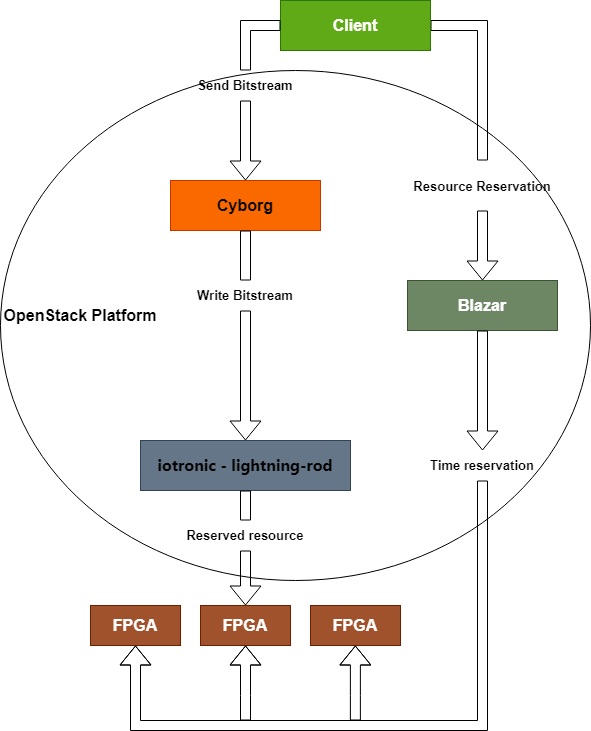
\includegraphics[width=0.45\textwidth]{images/Stack1.png}
\caption{Stack dell'architettura}
\end{figure}\clearpage
Un esempio applicativo potrebbe essere un laboratorio virtuale, dove ogni utente finale, professori, studenti o utenti privati, hanno accesso ad un'infrastruttura che presenta molte risorse cloud tra cui le FPGA, dove su di esse è possibile effettuare il caricamento del proprio bitstream precedentemente prodotto.\\
Ma più banalmente potrebbe esser visto come un sistema di prenotazione delle risorse per il Cloud Computing, portando ad un incremento di performance rispetto alle strutture classiche per via dell'uso delle FPGA, che tramite la loro riprogrammazione permettono una maggior flessibilità, una maggior potenza computazionale e soprattutto la divisione in regioni, la quale permette la possibilità di ospitare più acceleratori in un singolo device, permettendo cosi di avere più risorse virtuali disponibili all'utente, ma con lo stesso numero di board.\\
Le varie fasi del processo verranno effettuate da diversi servizi presenti nella piattaforma \textit{OpenStack}, il servizio che orchestra le risorse sarà \textit{Blazar}, come spiegato nella sotto sezione \ref{Blazar}, esso permette la \textit{Resource Reservation} tramite un altro servizio che effettua il WebServer sarà possibile invocare le API che permettono la reservation.
\begin{figure}[h]
\centering
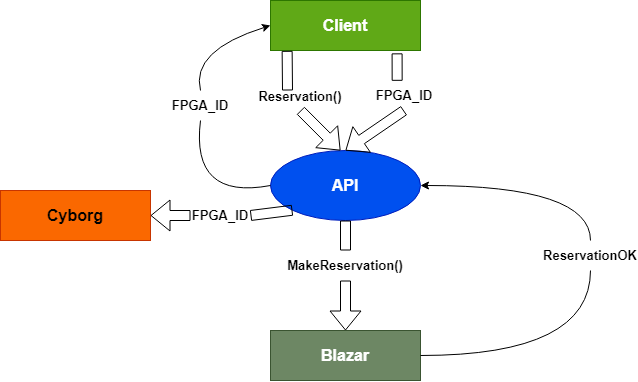
\includegraphics[width=0.4\textwidth]{images/Arch1.png}
\caption{Diagramma che rappresenta le fasi di reservation}
\end{figure}\\
Una volta avvenuta l'effettiva prenotazione l'utente finale tramite il servizio \textit{Cyborg}, esso gestisce il ciclo di vita degli acceleratori, tra cui le FPGA, permettendo tramite la sua integrazione con \textit{Nova}, di virtualizzare le FPGA e rendere disponibile la gestione da parte dell'utente dei nodi da quest'ultimo riservati. Al fine di creare il punto di contatto tra il cloud e i dispositivi IoT verranno usati in simbiosi IoTronic e Lightning-rod, essi sono integrabili nella piattaforma OpenStack e quindi interfacciabili tramite le API agli altri servizi già presenti nel sistema. Come per loro definizione IoTronic sarà l'agente che verrà eseguito lato cloud e tramite una connessione \textit{WAMP} con Lightning-rod, agente eseguito su di una distro Linux presente sulla FPGA SoC, permetteranno il trasferimento del file binario e l'esecuzione di tutti gli script necessari alla riprogrammazione.
\begin{figure}[h]
\centering
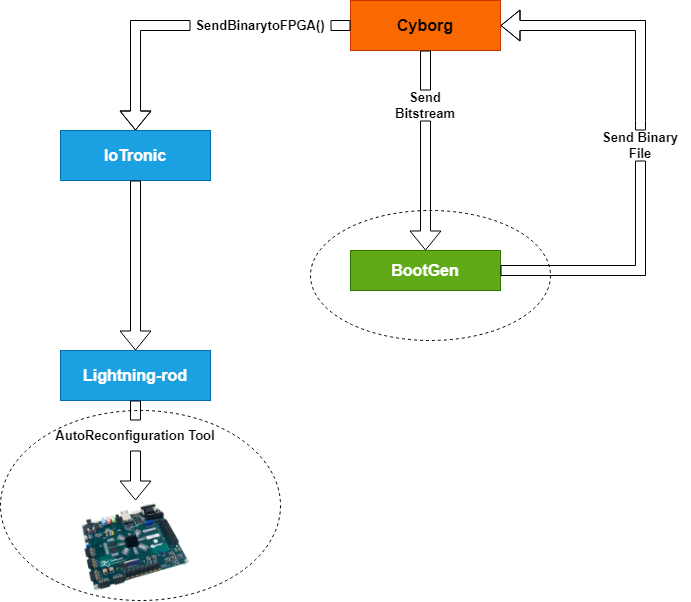
\includegraphics[width=0.6\textwidth]{images/Arch.png}
\caption{Diagramma che rappresenta le fasi post upload del bitstream}
\end{figure}\\
La scelta di fornire il bitstream e quindi aggiungere un livello di complessità in più ci permette di effettuare un analisi più accurata della validità del bitstream per l'architettura prenotata, tramite la decodifica del bitstream, infatti esso contiene informazioni riguardo la data di creazione, l'architettura e la dimensione, questo controllo permette di limitare gli errori che un utente novizio possa commettere riservando delle risorse non compatibili alla sua architettura.\\
Tutto il sistema è gestito dalle API di OpenStack, il quale ci garantisce questa integrazione tra servizi diversi tra di loro, rendendo il tutto trasparente all'utente finale.\\
In questa tesi verrà trattato il processo di automatizzazione per la generazione del file binario e per la riprogrammazione automatica tramite Lightning-rod.
 



\chapter{Interfacciamento IoT-Cloud con FPGA}
\label{Linux}
Il primo passaggio per l'integrazione delle FPGA SoC nel sistema IoT-Cloud è permettere l'interfacciamento con la rete tramite una distro Linux embedded, essa sarà montata sulla parte a microprocessore della board, al fine di permettere l'esecuzione dell'agente che effettuerà l'interfacciamento con il sistema Cloud e quindi garantire l'uso della risorsa nell'architettura precedentemente descritta.
\section{WorkFlow di Petalinux}
Come già visto nell'appendice \ref{InstPeta} petalinux è un tool della xilinix che ci permette di creare un kernel linux per sistemi FPGA SoC.\\
Petalinux tramite l'esportazione del hardware da vivado\footnote{\ref{ExportVivado}} ed un Board Support Package (BSP)\footnote{Esso rappresenta un codice di supporto di un implementazione per una determinata scheda} ci da la possibilità di creare il kernel per la scheda di riferimento.\\
Petalinux oltre a definire il kernel ed il comportamento degli stati di boot, ci permette di costruire il file system, in maniera puramente custom, tramite l'uso di Yocto, esso è un progetto open-source che permette alla community indipendentemente dall'architettura hardware.\\
Una volta effettuati i passaggi descritti nel \ref{SetupPeta}, è possibile effettuare tramite console linux l'effettiva creazione del kernel.
\subsection{Creazione di un progetto}
Al fine di creare un progetto è possibile percorrere due strade, usare un template\footnote{Nel caso di zedboard bisogna usare zynq} o l'uso di un BSP\footnote{\href{https://www.xilinx.com/member/forms/download/xef.html?filename=avnet-digilent-zedboard-v2021.2-final.bsp}{Xilinix}}.
\begin{lstlisting}[language=sh, label=lst:sh, caption={Comando creazione progetto con BSP}]
petalinux-create -t project -s <PATH-TO-BSP>
\end{lstlisting}
\begin{lstlisting}[language=sh, label=lst:sh, caption={Comando creazione progetto con il template}]
petalinux-create --type project --template <PLATFORM> --name <PROJECT_NAME> 
\end{lstlisting}
\begin{lstlisting}[language=sh, label=lst:sh, caption={Output atteso}]
INFO: Create project:
INFO: Projects:
INFO: * xilinx-zcu102-v<petalinux-version>
INFO: has been successfully installed to /home/user/
INFO: New project successfully created in /home/user/
\end{lstlisting}
Entrambe le scelte sono intercambiabili, poichè ci daranno solamente lo scheletro sulla quale poi modellare tutto il sistema.
\subsection{Configurazione del sistema}
Dopo la creazione dello scheletro è però necessario configurare il progetto in base alle esigenze progettuali, quindi al fine di far ciò sarà necessario muoversi nella cartella di progetto e definire l'hardware del progetto tramite l'hardware definition file\footnote{Xilinix Support Archive, XSA},  esso si può accumunare ad un archivio al cui interno ci sono tutte le informazioni necessarie per costruire la piattaforma per la struttura che è stata progetta antecedentemente\footnote{Per la progettazione si rimanda a \ref{CreazioneVivado}, mentre per l'export del file XSA a \ref{ExportVivado}}. Al suo interno troveremo le librerie PS7\footnote{Cambiano per ogni architettura}, Processing System 7000, come la nostra architettura, essi sono strettamente legali al processo di boot lato PS\footnote{Processing System}, nel dettaglio i file PS7\_init contengono tutte le configurazioni per il clock, la memoria ed il GPIO, inoltre essi vengono usati per creare il First Stage BootLoader (FSBL), il qui compito è quello di puntare al Second Stage BootLoader nella partizione di boot. 
\begin{lstlisting}[language=sh, label=lst:sh, caption={Comando necessario alla definizione dell'hardware}]
petalinux-config --get-hw-description <PATH-TO-XSA Directory>/<PATH-TO-XSA>
\end{lstlisting}
Questo passaggio risulta essere critico ai fini del proseguio corretto dello sviluppo, poichè un errata esportazione del file XSA o l'incompatibilità del sistema operativo con il tool potrebbero causare errori.\\
Nel caso in cui questo passaggio sia andato a buon fine, si presenterà la seguente schermata
\begin{figure}[h]
\centering
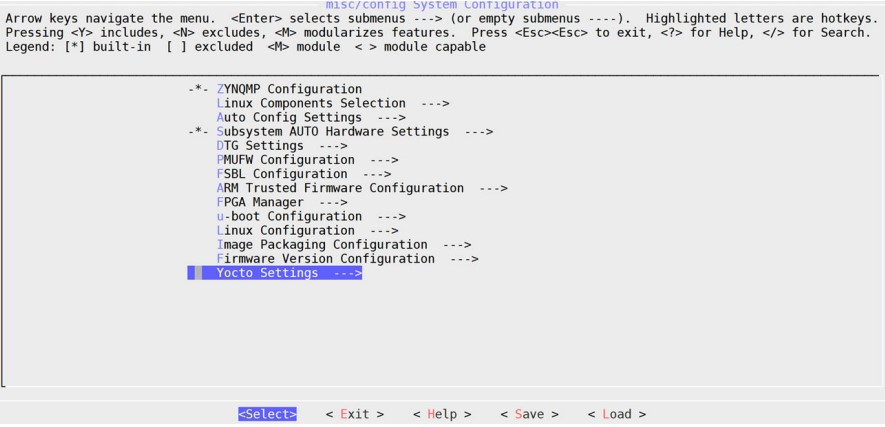
\includegraphics[width=0.9\textwidth]{images/image1.jpg}
\caption{Schermata di configurazione del sistema}
\end{figure}
Ai fini della tesi sarà necessario abilitare il parametro FPGA Manager, che trattato nel dettaglio al capitolo \ref{chap:Cap3}.\\
Dopo aver configurato l'hardware e quindi i parametri del boot loader\footnote{U-BOOT}, è necessario riconfigurare il file system ed eventualmente il kernel.
\begin{lstlisting}[language=sh, label=lst:FileSystem, caption={Comando necessario alla riconfigurazione del file system}]
petalinux-config -c rootfs

\end{lstlisting}
Se il comando è andato a buon fine comparirà la seguente schermata
\begin{figure}[h]
\centering
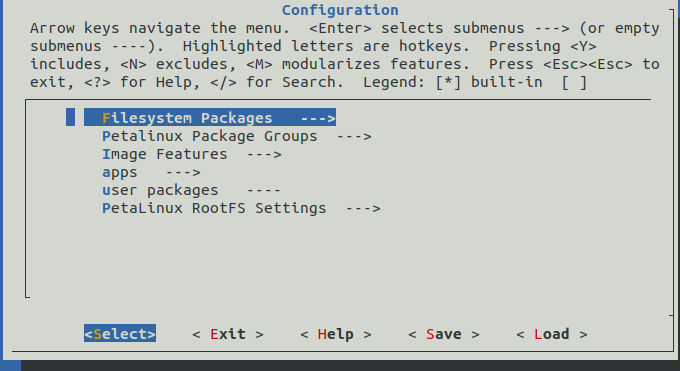
\includegraphics[width=0.9\textwidth]{images/peta1.png}
\caption{Schermata di modifica file system}
\end{figure}
Da qui sarà possibile attivare o disattivare packages, al fine della programmazione on-board e per un ottimale interfacciamento con il sistema cloud è fortemente consigliato abilitare i seguenti package:
\begin{itemize}
    \item \textit{Petalinux Package Groups -> packagegroup-petalinux-utils}, al fine di avere GCC per l'architettura ARM Cortex A9.
    \item \textit{Petalinux Package Groups -> packagegroup-petalinux-python} e \textit{Filesystem Packages-> devel-> Python}, al fine di avere l'interprete di Python.
    \item \textit{console-> utils -> git}, al fine di avere il comando git.
\end{itemize}
Terminato ciò si potrà passare alla modifica del kernel, questa modifica risulta necessaria per poter effettuare le attività di tesi.
\begin{lstlisting}[language=sh, label=lst:sh, caption={Comando necessario alla riconfigurazione del kernel}]
petalinux-config -c kernel
\end{lstlisting}
Dalla schermata, che sarà analoga a quelle precedenti, è necessario abilitare i seguenti moduli\footnote{Per "[*]" si intende selezionato e si fa posizionandosi sopra il modulo desiderato e premendo la barra spaziatrice}:
\begin{itemize}
    \item \textit{Device Drivers ---> FPGA Configuration Framework -> [*]FPGA Region}, l'FPGA Region verrà discussa nel dettaglio nel capitolo \ref{cap5}
    \item \textit{Device Drivers ---> FPGA Configuration Framework -> [*]FPGA Bridge Framework}, il Bridge verrà discusso nel dettaglio nel capitolo \ref{cap5}
    \item \textit{Device Drivers --> Device Tree and Open Firmware support -> [*] Device Tree Overlays}, il suo scopo è modificare il device tree del kernel mentre è in esecuzione, una sua modifica si ripercuote sul lato FPGA, causandone una modifica.
    \item \textit{Device Drivers --> Device Tree and Open Firmware support -> [*] Device Tree Overlays ConfigFS Interface}
    \item \textit{Memory Management options ---> [*] Contiguous Memory Allocator}, il Contiguous Memoy Allocator verrà discusso nel dettaglio nel capitolo \ref{comunicazioneCap}
    \item \textit{Library routines--> DMA Contiguous Memory Allocator }
\end{itemize}

\section{Creazione app e modulo kernel}
Creare un app a livello kernel può risultare comodo, al fine di creare l'applicazione ed innestarla al nostro file system sarà necessario eseguire il seguente comando:
\begin{lstlisting}[language=sh, label=lst:creazioneApp, caption={Comando necessario alla creazione dell'applicazione, va eseguito nella cartella del progetto}]
petalinux-create -t apps --name [nome desiderato] --template [c, c++, autoconf, install]
\end{lstlisting}
Se il comando è stato eseguito correttamente il codice per l'applicazione si troverà nella cartella 
\textit{/project-spec/meta-user/recipes-apps/Nome Desiderato}.
\subsection{Compilazione}
Prima di poter compilare l'applicazione sarà necessario aggiungerla al file system, eseguendo i comandi visti nel codice \ref{lst:FileSystem}, spostandoci nel menu \textit{apps -> [nome desiderato]} sarà possibile selezionarlo.\\
Effettuato ciò per compilare è necessario eseguire:
\begin{lstlisting}[language=sh, label=lst:sh, caption={Comando necessario alla compilazione dell'applicazione}]
petalinux-build -c [nome desiderato]
\end{lstlisting}
\subsection{Modulo kernel}
Ai fini della creazione del modulo per il kernle, sarà necessario eseguire alcuni comandi:
\begin{lstlisting}[language=sh, label=lst:sh, caption={Comando necessario alla creazione del modulo kernel}]
petalinux-create -t modules --name [nome desiderato] --enable
\end{lstlisting}
Analogalmente all'applicazione il modulo si troverà nella cartella \textit{/project-spec/meta-user/recipes-modules/[nome desiderato]}, esso sarà compilato una volta compilato il kernel.

\section{Compilazione kernel}
Una volta ultimata la progettazione e la configurazione del kernel e del file system è necessaria la compilazione al fine di generare il codice binario, in ambiente petalinux sarà necessario usare il comando
\begin{lstlisting}[language=sh, label=lst:sh, caption={Comando necessario alla compilazione del kernel}]
petalinux-build
\end{lstlisting}
Questo passaggio sarà onesoro temporalmente, poichè si dovranno linkare tutte le librerie ed eventualmente scaricare moduli aggiunti in fase di configurazione.
\subsection{Pacchettizzazione del kernel}
Una volta che il kernel è compilato nella cartella \textit{images/linux} si troveranno tutte le componenti del sistema operativo. Quindi eseguendo il seguente comando
\begin{lstlisting}[language=sh, label=lst:sh, caption={Comando necessario alla pacchettizzazione del kernel}]
petalinux-package -boot -format BIN -fsbl image/linux/[FSBL] -fpga <path/to/bitstream> -u-boot
\end{lstlisting}

\chapter{Interfaccia Soft Core - Gate Array}
\label{comunicazioneCap}
Nell'ambiente delle FPGA SoC è importante garantire l'alta performace e la bassa latenza. \textit{Processing System} e \textit{Programmable Logic} comunicano tra di loro al fine di permettere il corretto funzionamento della scheda alle sue massime funzionalità.\\
Tuttavia il metodo di interfacciamento tra le due aree non è univoco. In questo capitolo verrà trattato il metodo più comune e diffuso tra quelli disponibili in tutte le FPGA SoC.
\section{Interfacce di comunicazione}
Le ZYNQ-7000 usano diversi metodi di comunicazione tra PS e PL, tutte basate su tecniche di interconnessione, le interfacce possono essere suddivise in due categorie\cite{Doc}:
\begin{itemize}
    \item Functional Interface, le quali rientrano l'AXI, i controller DMA e la Extended MIO.
    \item Configuration Signals, contenente il Processor Configuration Access Port che verrà approfondito nel capitolo \ref{cap5}.
\end{itemize}
Per la comunicazione tra PS e PL è preferibile usare il protocollo AXI, per via della sua diffusione, compatibilità e velocità.
\section{Advanced Microcontroller Bus Architecture, AMBA}
Prima di parlare del protocollo AXI, è necessario esporre il protocollo AMBA, esso è un open-standard per la comunicazione nei system-on-chip SoC. AMBA definisce come i blocchi funzionali comunicano tra di loro, definendo il tutto nel Device Tree,\cite{amba}
\begin{lstlisting}[language=sh, label=lst:C, caption={Questo è un esempio di un device tree che definisce la comunicazione di un core propretario tramite il protocollo CANBus.}]
  amba: amba {
          compatible = "simple-bus";
          #address-cells = <2>;
          #size-cells = <2>;
          ranges;
          can0: can@ff060000 {
                     compatible = "xlnx,zynq-can-1.0";
                     clock-names = "can_clk", "pclk";
                     reg =<0x0 0xff060000 0x0 0x1000>;
          };
  };
\end{lstlisting}
\begin{figure}
    \centering
    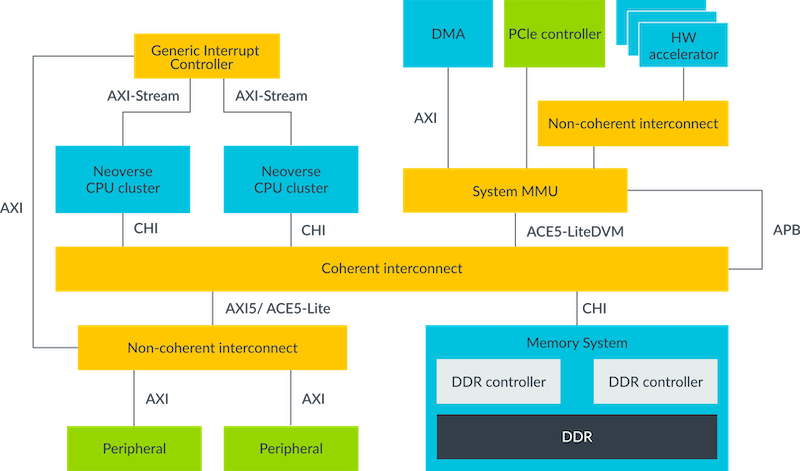
\includegraphics[width=0.7\textwidth]{images/AMBA.png}
    \caption{Diagramma raffigurante SoC, tutti i collegamenti saranno decisi dal protocollo AMBA, si può notare come figura il protocollo AXI\cite{amba}}
    \label{fig:my_label}
\end{figure}
\subsection{Perchè e dov'è usato AMBA}
Il protocollo AMBA è usato per semplificare lo sviluppo di schede contenenti più processori e un grande numero di periferiche e controllori.\\
È diventato uno standard data la sua flessibilità, compatibilità, larghezza di banda e latenza.
\section{Advanced eXtensible Interface}
È un protocollo di interfaccia sviluppato sulle architetture ARM e parte del protocollo AMBA.
\begin{figure}
    \centering
    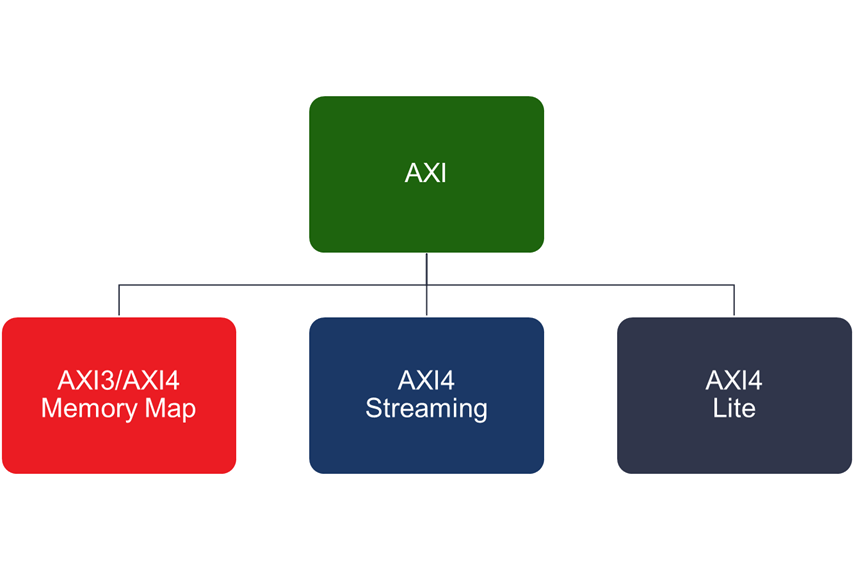
\includegraphics[width=0.5\textwidth]{images/AXI1.png}
    \caption{I 3 tipi d'interfaccia AXI}
    \label{fig:my_label}
\end{figure}
L'AXI è un protocollo master-slave, usato per connessioni con periferiche e memorie, essendo presenti più master in base alle priorità si determina quale master potrà usare il bus, mentre un decodere eseguirà la selezione dello slave.\\
Le operazioni sono eseguite in burst, solitamente da 256bit, che può richiedere più cicli di clock per esser completata, ogni burst consiste in due fasi, la prima di indirizzamento e la seconda di scambio dati, fornendo elevate prestazioni per accessi di tipo memory mapped.\\
È composto da 5 canali indipendenti tra master e slave\cite{AXI} :
\begin{itemize}
    \item Write Address 
    \item Write Data
    \item Read Address
\end{itemize}
Quelli direzione Master to Slave, mentre Slave to Master:
\begin{itemize}
    \item Write Response
    \item Read Data
\end{itemize}
\begin{figure}
    \centering
    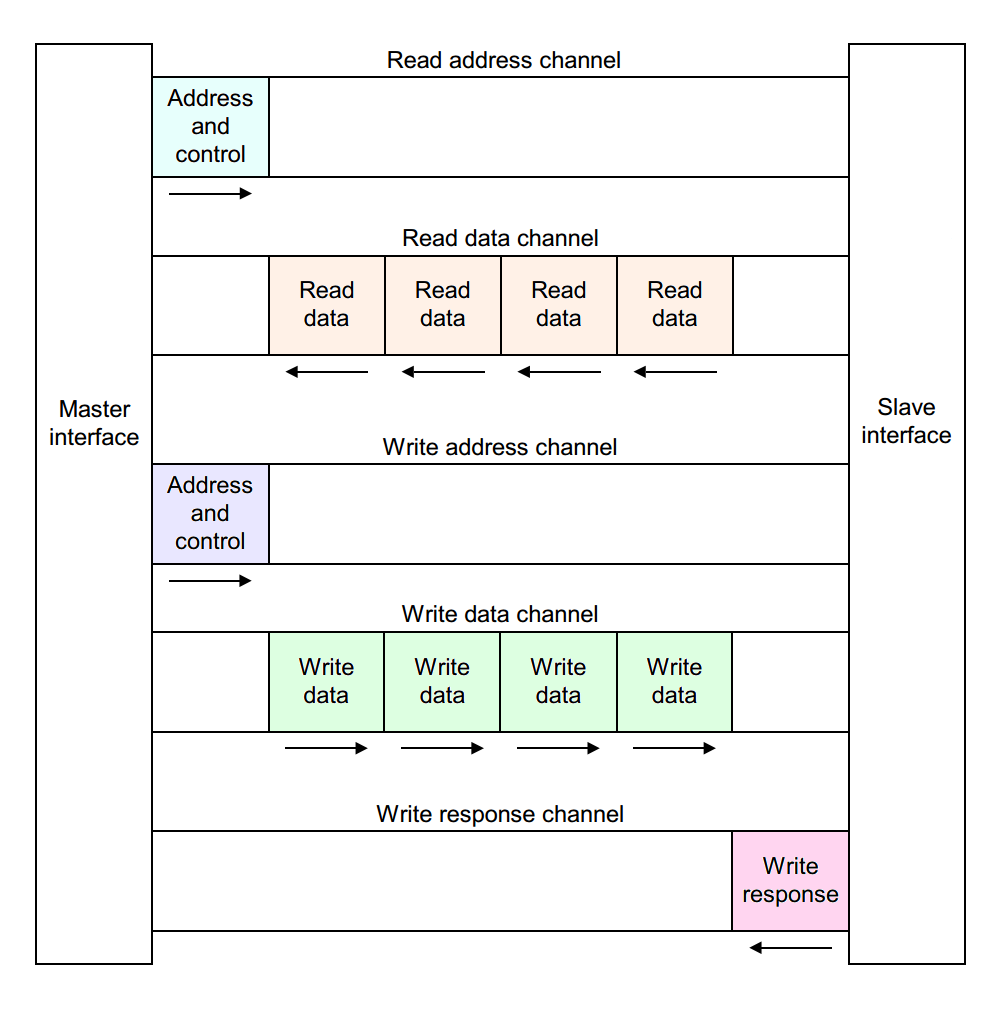
\includegraphics[width=0.9\textwidth]{images/AXI2.jpg}
    \caption{Esempio di comunicazione tramite protocollo AXI, i blocchi multipli stanno ad identificare i Burst}
    \label{fig:my_label}
\end{figure}
I dati possono viaggiare simultaneamente in entrambe le direzioni, esso è possibile per via delle due connessioni separate, in indirizzi e dati, sia per lettura che per scrittura. Ogni scambio di dati è detto transazione essa include l'indirizzo, le informazioni di controllo, i dati inviati e qualsiasi informazione di risposta.
\subsection{AXI nei sistemi ZYNQ}
Nell'architettura ZYNQ-7000, ma come tutte le architetture ZYNQ, il protocollo AXI permette l'interfacciamento tra Processing System (PS) e Programmable Logic (PL).
\begin{figure}
    \centering
    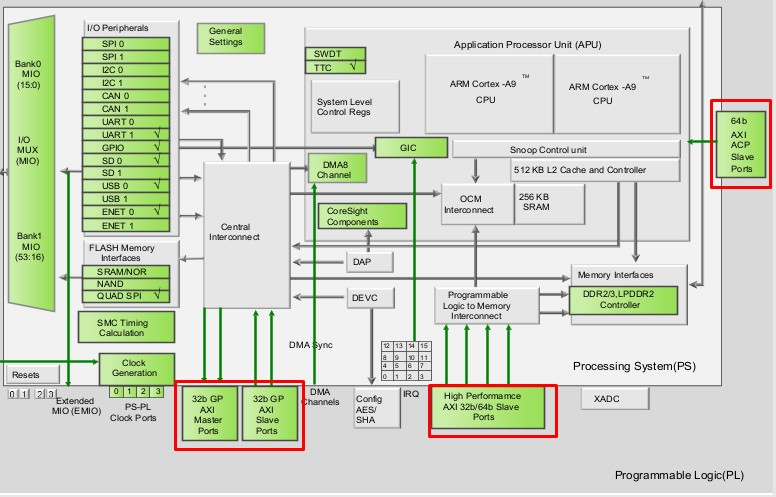
\includegraphics[width=0.9\textwidth]{images/AXI3.jpg}
    \caption{Design di un architettura ZYNQ-7000, dove sono evidenziati i blocchi AXI}
    \label{fig:my_label}
\end{figure}
\begin{figure}
    \centering
    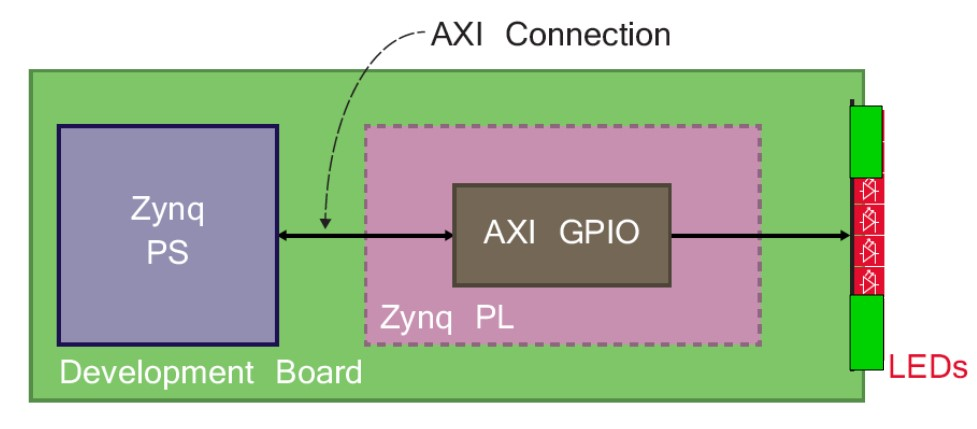
\includegraphics[width=0.7\textwidth]{images/axi.jpg}
    \caption{Zoom della connessione tra PS e PL}
    \label{fig:my_label}
\end{figure}\\
In quest'architettura abbiamo delle interfacce di comunicazione sul bus AXI.
Al fine di facilitare lo sviluppo della scheda la xilnix ha prodotto un componente, completamente riprogrammabile, detto AXI Interconnect, esso facilità e gestisce tutte le connessioni tra master e slave.\clearpage
\begin{figure}
    \centering
    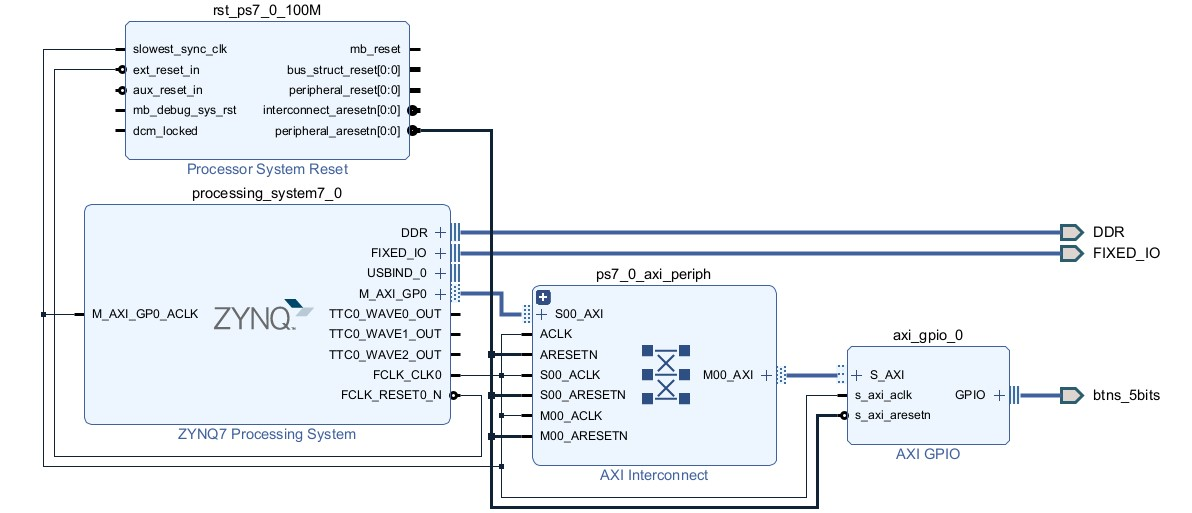
\includegraphics[width=0.9\textwidth]{images/AXI4.jpg}
    \caption{Schema contentente l'interconnecter}
    \label{fig:my_label}
\end{figure}
\subsection{Comunicazione memory-mapped tra PS e PL}
Al fine di far comunicare tramite gli indirizzi definiti in fase di progettazione dobbiamo usare il Central Direct Memory Access (CDMA), esso è un core prodotto da Xilnix che ci permette di avere una connessione tra una sorgente con un indirizzo memory-mapped  ed una destinazione con un indirizzo memory-mapped, tramite il protocollo AXI. Quindi è in grado di associare un indirizzo mappato in memoria fisica con un indirizzo mappato in memoria logica, evitando cosi il vincolo imposto dal sistema operativo sull'accesso agli indirizzi fisici tramite la funzione mmap. \clearpage
\begin{figure}
    \centering
    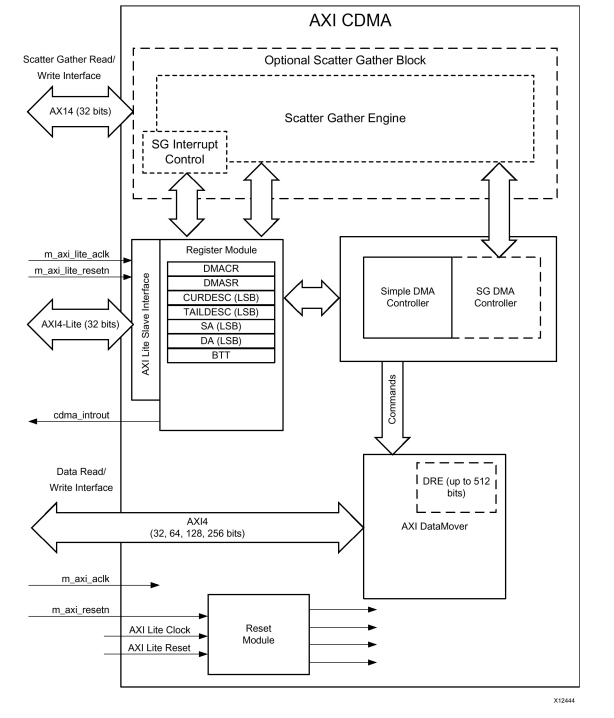
\includegraphics[width=0.8\textwidth]{images/AXI6.jpg}
    \caption{Schema del CDMA}
    \label{fig:my_label}
\end{figure}

Nel caso di un FPGA SoC con un Real Time OS (RTOS), può esser usata per interfacciarsi con il GPIO lato FPGA, con dei core di calcolo tensoriale o per la riprogrammazione sia completa che parziale della PL.
\section{Driver AXI}
Andremo a programmare, leggere e manipolare i dati presenti nella Programmable Logic ed interconnessi con la PS tramite il protocollo AXI e sfruttando il core CDMA ed il funzionamento di esso
\begin{figure}
    \centering
    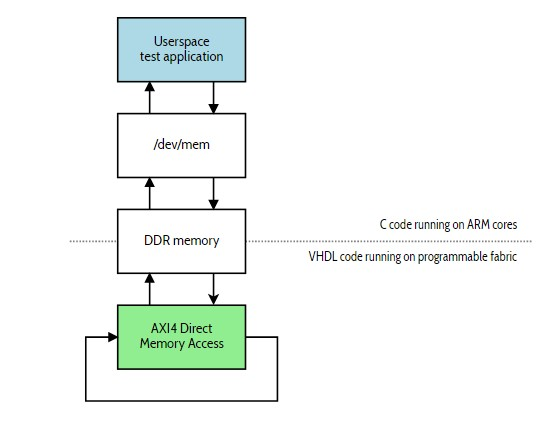
\includegraphics[width=0.7\textwidth]{images/AXI7.jpg}
    \caption{Funzionamento minimo del CDMA}
    \label{fig:my_label}
\end{figure}\\
Il driver necessita di conoscere gli indirizzi base dei core interconnessi al protocollo AXI e la loro dimensione ed eventuale offset.
\begin{lstlisting}[language=C, label=lst:C, caption={Definizione costanti}]
    #define GPIO_BASE_ADDRESS       0x42000000
    #define GPIO_MAP_SIZE           0x1000
    #define XAXIGPIO_DATA_OFFSET    0x00000000
\end{lstlisting}
Poichè necessitiamo di usare \textit{/dev/mem/}, file che rappresenta l'immagine della memoria centrale del microprocessore, per effettuare l'associazione tra indirizzo fisico noto ed indirizzo logico, dobbiamo andare ad effettuare un'apertura assicurandoci che sia andato a buon fine
\begin{lstlisting}[language=C, label=lst:C, caption={Apertura file mem}]
    int memfd;
    if ( (memfd = open("/dev/mem", O_RDWR | O_DSYNC)) == -1 ){
        printf("Can't open /dev/mem.\n");
        exit(-1);
    }
\end{lstlisting}
Una volta effettuato ciò potremmo andare accedere, tramite la funzione mmap all'indirizzo del core AXI con la quale vogliamo interfacciarci, quest'apertura dovra esser sia in lettura che scrittura e map shared, quindi visibile anche a tutti i processi mappati nella stessa regione, quindi usiamo
\begin{lstlisting}[language=C, label=lst:C, caption={Mapping dell'indirizzo di GPIO}]
    void *gpioMapAddr = NULL;
    gpioMapAddr = mmap(0, GPIO_MAP_SIZE, PROT_READ | PROT_WRITE, MAP_SHARED, memfd, GPIO_BASE_ADDRESS);
    if (gpioMapAddr == (void *) -1){
        printf("Can't map the CDMA-Control-Port to user space.\n");
        exit(-1);
    }
\end{lstlisting}
Se il tutto ha avuto esito positivo possiamo effettuare la manipolazione dei dati presenti in esso, andando a sommare l'eventuale offset e l'indirizzo fornitoci dalla funzione mmap
\begin{lstlisting}[language=C, label=lst:C, caption={Esempio con un contatore tramite i led}]
    unsigned long ii;
    for(ii=0; ii<256; ii++){
        *((volatile unsigned long*) (gpioMapAddr + XAXIGPIO_DATA_OFFSET)) = ii;
        printf("led = 0x%02x\n", ii);
        usleep(20000); // sleep 20ms
    }
\end{lstlisting}
Questo esempio può esser modificato ad hoc al fine di accedere ai core interconnessi con il protocollo AXI, questo da la base alla partial reconfiguration tramite due controller già presenti nei SoC. Questo codice può esser compilato sia on-board, sia tramite la cross compilazione, per la cross compilazione si rimanda a \ref{crossComp}\clearpage



\chapter{Gate Array Reconfiguration}
\label{chap:Cap3}
\section{Full Reconfiguration}
La riprogrammabilità delle FPGA è la chiave per la loro adozione nei sistemi Cloud. In tal modo l'FPGA risulterà essere un sistema versatile, scalabile, efficiente ed ottimo per il cloud computing. Per la riprogrammazione delle FPGA SoC è possibile eseguire delle procedure automatiche, e non, per la riprogrammazione completa della Programmable Logic.

\subsection{FPGA Manager}
Esso bisogna che sia abilitato nella struttura del kernel, poichè è un insieme di API agnostiche che la loro chiamata ci permette di programmare, o riprogrammare, l'FPGA tramite un file binario.
\subsection{Creazione del file binario}
Per la creazione del file binario, si necessita un bitstream la quale generazione è discussa nell'appendice \ref{ExportVivado}.\\
Questa procedura necessita del tool bootgen, si rimanda a \ref{installazioneBoot} per l'installazione, il quale al fine di generare il file binario necessità uno file intermedio il Boot Image Format (BIF), questo file è cosi strutturato:
\begin{lstlisting}[language=sh, label=lst:C, caption={template file .bif}]
all:{./path/bitstream.bit}
\end{lstlisting}
Il file solitamente contiene tutte le fasi di boot ed eventuali partizioni dell'immagine.\\
Al termine di ciò sarà necessario caricare l'environment di lavoro di bootgen, semplicemente spostandosi nella cartella d'installazione ed eseguendo il seguente:
\begin{lstlisting}[language=sh, label=lst:C, caption={setup environment bootgen}]
source  settings64.sh
\end{lstlisting}
In questo modo tramite il comando 
\begin{lstlisting}[language=sh, label=lst:C, caption={setup environment bootgen}]
bootgen -image [/path/to/bifFile] -arch zynq -process_bitstream bin
\end{lstlisting}
All' appendice \ref{autoBOOT} è disponibile uno script in grado di automatizzare questo processo.
\section{Invocazione classe FPGA Manager}
Dopo la generazione del file binario, esso andrà copiato nella scheda SD in una qualsiasi partizione.\\
Al fine di abilitare la riprogrammazione completa della scheda sarà sfruttata la classe FPGA Manager, essa per l'abilitazione necessità alcuni comandi da eseguire all'interno della scheda\cite{PL}:
\begin{lstlisting}[language=sh, label=lst:C, caption={Abilitazione FPGA\_manager}]
echo 0 > /sys/class/fpga_manager/fpga0/flags
\end{lstlisting}
Questo comando imposta le Flags dell'fpga manager per accettare un nuovo bistream, quindi di fatto abilitando la riprogrammazione.\\
Di seguito bisognerà caricare il bitstream nella Programmable Logic
\begin{lstlisting}[language=sh, label=lst:C, caption={Caricamento bitstream nella Programmable Logic}]
mkdir -p /lib/firmware
cp [NomeBIN.bin] /lib/firmware/
\end{lstlisting}
Infine per effettuare la completa riprogrammazione è necessario puntare il nuovo file binario caricato nella PL, per far ciò è necessario comunicarlo al FPGA\_Manager
\begin{lstlisting}[language=sh, label=lst:C, caption={Comunicazione nuovo bitstream alla PL}]
echo [NomeBIN.bin] > /sys/class/fpga_manager/fpga0/firmware
\end{lstlisting}
La verifica dell'avvenuta riprogrammazione è visibile tramite un led on-board o tramite l'esecuzione di un sorgente che sfrutta il driver GPIO precedentemente discusso al capitolo \ref{comunicazioneCap}.\\
All'appendice \ref{Riprogrammazione} è possibile trovare uno script automatico per la riprogrammazione.
\section{Partial Reconfiguration}
Le FPGA, oltre la loro riprogrammazione, si rendono ancora più versatili tramite l'uso delle regioni. Quest'ultime rappresentano una parte di FPGA che può esser riprogrammata senza intaccare il resto della board, permettendo di avere molteplici acceleratori.\\
Le regioni definite nel seguente modo
\begin{figure}
    \centering
    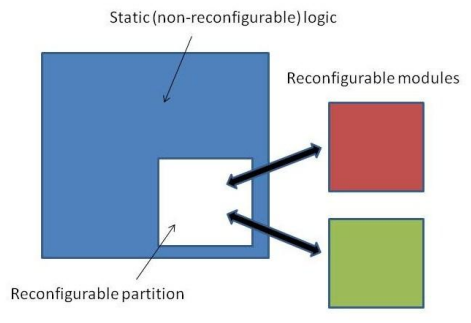
\includegraphics[width=0.4\textwidth]{images/PR1.png}
    \caption{Definizione regioni FPGA}
    \label{fig:my_label}
\end{figure}\\
Non tutte le regioni sono riprogrammabili, ma solo alcune. Queste vengono dette \textit{Partially Reconfigurable Region} (PRR). Questo modo di definire le FPGA rende ancora più conveniente la loro integrazione in un sistema IoT-Cloud.
\subsection{Place and Route per il Partial Bitstream}
La creazione di un Partial Bitstream, parte prima dalla progettazione dell'hardware, dove dovremmo descrivere, tramite Verilog o VHDL, un Intellectual Property(IP)\cite{PRRGIT}, un soft core che sia una blackbox, tramite essa sarà possibile effettuare il \textit{floorplanning}, esso è un tentativo di rappresentazione di come saranno piazzati i blocchi funzionali.
\begin{figure}
    \centering
    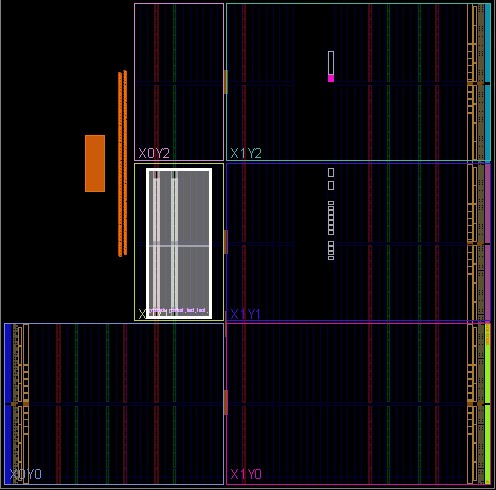
\includegraphics[width=0.4\textwidth]{images/Floor1.jpg}
    \caption{FloorPlanning in un FPGA Xilinx}
    \label{fig:my_label}
\end{figure}\\
Effettuato ciò potremmo effettuare il \textit{Place and Route}, generando cosi l'implementazione della scheda al fine di generare il \textit{Bitstream}\cite{PRR}. 
\subsection{Interfaccia per la riconfigurazione parziale}
Le FPGA SoC permettono la programmazione della Programmable Logic tramite il Processing System, esso si interfaccerà tramite l'interfaccia \textit{Device Configuration interface}(DevC), essa possiede un'interfaccia DMA che tramite il bus AXI trasferirà il partial bitstream ad una delle due \textit{Configuration Access Port}, rispettivamente \textit{Processor Configuration Access Port}(PCAP) e \textit{Internal Configuration Access Port} (ICAP).
\begin{figure}
    \centering
    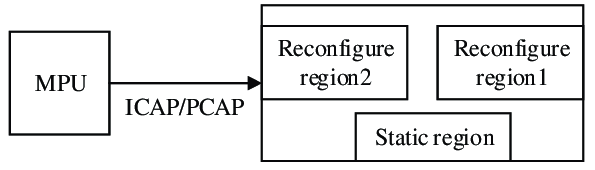
\includegraphics[width=0.4\textwidth]{images/PRR.png}
    \caption{Esempio di interfacciamento tra PS e PL per la riprogrammazione\cite{PRR2}}
    \label{fig:my_label}
\end{figure}\\
La loro coesistenza non è permessa dall'architettura, è possibile lo scambio tra le due interfacce anche runtime, tramite la modifica di un registro interno alla Processing System.\\
La Xilinix garantisce un IP core \textit{AXI$\_$HWICAP}, che abilita la \textit{Partial Reconfiguration} tramite l'uso di \textit{ICAP}. Il processo di riprogrammazione parziale è stato svolto tramite l'uso di un controller chiamato \textit{ZyCap}\cite{PRR}
\begin{figure}
    \centering
    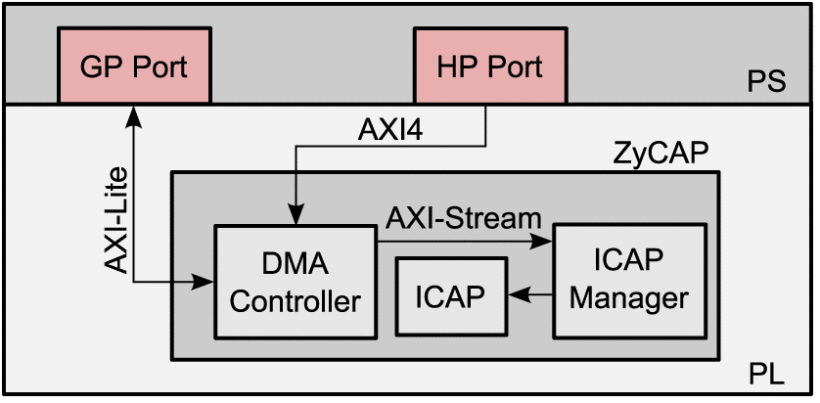
\includegraphics[width=0.4\textwidth]{images/ZyCap.png}
    \caption{Interfaccia tra PS e PL con il controller}
    \label{fig:my_label}
\end{figure}
\section{Problemi e possibili soluzioni}
Sfortunatamente l'architettura scelta al fine della realizzazione della tesi non supportava nativamente la \textit{Partial Reconfiguration}, rendendo impossibile la realizzazione di quest'ultima, anche causa un'obsoleta letteratura scientifica.\\
Il principale problema è dovuto dalla non completa integrazione di vivado con i meccanismi di sviluppo dei partial bitstream, poichè risulta impossibile esportare la definizione del hardware contenente tutte le informazioni inerenti al FPGA appena progettata, qualora si riuscisse ad esportare il file XSA sarà necessario creare il progetto su Vitis, ma le librerie usate in \cite{PRR} sono buona parte deprecate, rendendo inutile il processo di progettazione del codice per la riprogrammazione.\\
\subsection{Possibili soluzioni}
Alcuni possibili soluzioni potrebbero essere il cambio di architettura come ad esempio il passaggio a \textit{ZynqMP}, ma anche la creazione di un nuovo controller sulla base del \textit{Zycap}, quindi usando un \textit{AXI DMA} ed un controller per gli \textit{ICAP}. Ovviamente la creazione di un nuovo controller comporta la riscrittura del driver di riprogrammazione, che per alcuni tratti può esser basato su quello usato per il controllo del bus AXI, il driver dovrà necessariamente interfacciarsi con l'interfaccia \textit{DevC}, la quale però viene astratta tramite una libreria già fornita dalla Xilinix.\\
Il metodo appena descritto può esser usato per effettuare una riprogrammazione BareMetal, quindi senza la presenza di un sistema operativo lato PS, questo comporta l'introduzione di un elemento in più, assimilabile ad un raspberry, che ospiterà l'agente Lightning-rod per la connessione al cloud.



%\chapter{Gate Array Partial Reconfiguration}
\label{cap5}
Le FPGA oltre la loro riprogrammazione, già vista nel capitolo precedente, si rendono ancora più versatili tramite l'uso delle regioni, esse rappresentano una parte di FPGA che può esser riprogrammata senza intaccare il resto della board, questo permette di avere molteplici acceleratori.\\
Le regioni definite nel seguente modo
\begin{figure}
    \centering
    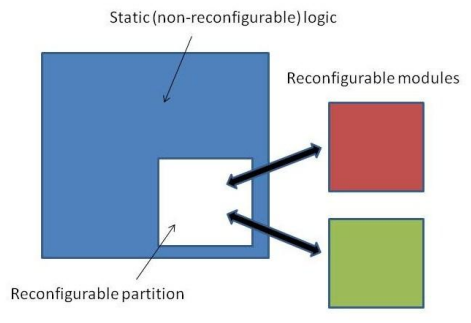
\includegraphics[width=0.4\textwidth]{images/PR1.png}
    \caption{Definizione regioni FPGA}
    \label{fig:my_label}
\end{figure}\\
Non tutte le regioni però sono riprogrammabili, ma solo alcune che vengono dette \textit{Partially Reconfigurable Region} (PRR). Questo modo di definire le FPGA rende ancora più conveniente la loro integrazione in un sistema IoT-Cloud.
\section{Place and Route per il Partial Bitstream}
La creazione di un Partial Bitstream, parte prima dalla progettazione dell'hardware, dove dovremmo descrivere, tramite Verilog o VHDL, un Intellectual Property(IP)\cite{PRRGIT}, un soft core che sia una blackbox, tramite essa sarà possibile effettuare il \textit{floorplanning}, esso è un tentativo di rappresentazione di come saranno piazzati i blocchi funzionali.
\begin{figure}
    \centering
    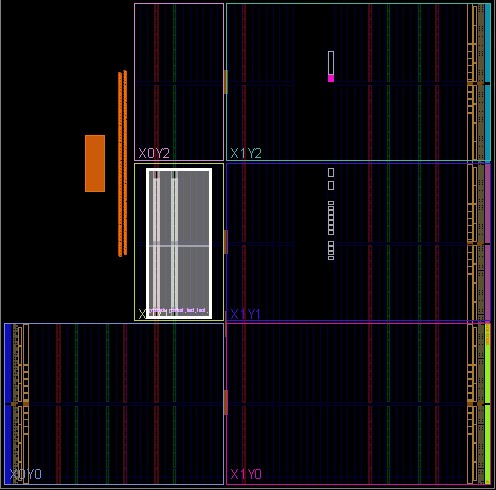
\includegraphics[width=0.4\textwidth]{images/Floor1.jpg}
    \caption{FloorPlanning in un FPGA Xilinx}
    \label{fig:my_label}
\end{figure}\\
Effettuato ciò potremmo effettuare il \textit{Place and Route}, generando cosi l'implementazione della scheda al fine di generare il \textit{Bitstream}\cite{PRR}. 
\section{Interfaccia per la riprogrammazione}
Le FPGA SoC permettono la programmazione della Programmable Logic tramite il Processing System, esso si interfaccerà tramite l'interfaccia \textit{Device Configuration interface}(DevC), essa possiede un'interfaccia DMA che tramite il bus AXI trasferirà il partial bitstream ad una delle due \textit{Configuration Access Port}, rispettivamente \textit{Processor Configuration Access Port}(PCAP) e \textit{Internal Configuration Access Port} (ICAP).
\begin{figure}
    \centering
    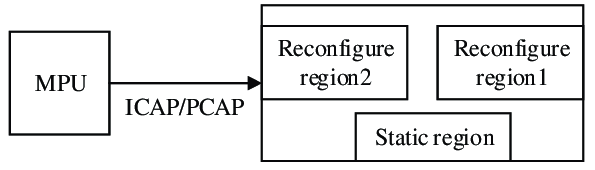
\includegraphics[width=0.4\textwidth]{images/PRR.png}
    \caption{Esempio di interfacciamento tra PS e PL per la riprogrammazione\cite{PRR2}}
    \label{fig:my_label}
\end{figure}\\
La loro coesistenza non è permessa dall'architettura, è possibile lo scambio tra le due interfacce anche runtime, tramite la modifica di un registro interno alla Processing System.\\
La Xilinix garantisce un IP core \textit{AXI$\_$HWICAP}, che abilita la \textit{Partial Reconfiguration} tramite l'uso di \textit{ICAP}. Il processo di riprogrammazione parziale è stato svolto tramite l'uso di un controller chiamato \textit{ZyCap}\cite{PRR}
\begin{figure}
    \centering
    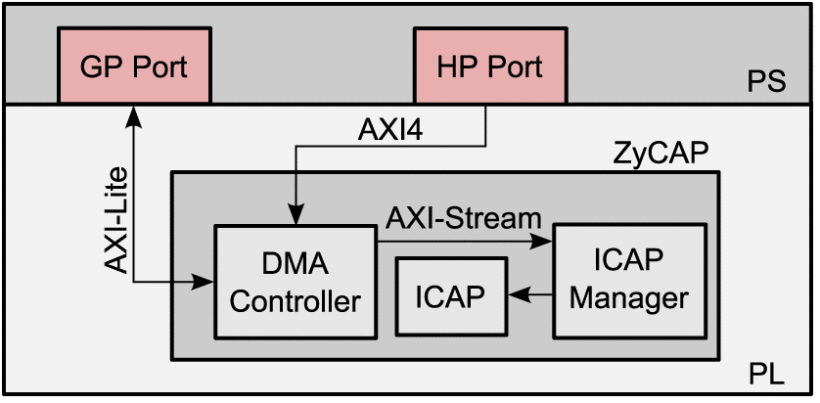
\includegraphics[width=0.4\textwidth]{images/ZyCap.png}
    \caption{Interfaccia tra PS e PL con il controller}
    \label{fig:my_label}
\end{figure}\\
\section{Problemi e possibili soluzioni}
Sfortunatamente l'architettura scelta al fine della realizzazione della tesi non supportava nativamente la \textit{Partial Reconfiguration}, rendendo impossibile la realizzazione di quest'ultima, anche causa un'obsoleta letteratura scientifica.\\
Il principale problema è dovuto dalla non completa integrazione di vivado con i meccanismi di sviluppo dei partial bitstream, poichè risulta impossibile esportare la definizione del hardware contenente tutte le informazioni inerenti al FPGA appena progettata, qualora si riuscisse ad esportare il file XSA sarà necessario creare il progetto su Vitis, ma le librerie usate in \cite{PRR} sono buona parte deprecate, rendendo inutile il processo di progettazione del codice per la riprogrammazione.\\
\subsection{Possibili soluzioni}
Alcuni possibili soluzioni potrebbero essere il cambio di architettura come ad esempio il passaggio a \textit{ZynqMP}, ma anche la creazione di un nuovo controller sulla base del \textit{Zycap}, quindi usando un \textit{AXI DMA} ed un controller per gli \textit{ICAP}. Ovviamente la creazione di un nuovo controller comporta la riscrittura del driver di riprogrammazione, che per alcuni tratti può esser basato su quello usato per il controllo del bus AXI, il driver dovrà necessariamente interfacciarsi con l'interfaccia \textit{DevC}, la quale però viene astratta tramite una libreria già fornita dalla Xilinix.\\
Il metodo appena descritto può esser usato per effettuare una riprogrammazione BareMetal, quindi senza la presenza di un sistema operativo lato PS, questo comporta l'introduzione di un elemento in più, assimilabile ad un raspberry, che ospiterà l'agente Lightning-rod per la connessione al cloud.



\chapter{Conclusioni}
\label{chap:conclusioni}
L'obiettivo di questo elaborato era quello di creare degli strumenti che permettessero l'interfacciamento al \textit{Cloud} e la riprogrammazione completa e parziale dell'\textit{FPGA}.\\
Lungo la trattazione è stato dimostrato come l'integrazione tra il sistema \textit{Cloud} e le \textit{FPGA} sia possibile e come la loro completa riprogrammazione sia effettuabile ed automatizzabile.\\
\\
Purtroppo non è stato possibile raggiungere quest'obiettivo.\\ L'implementazione di un meccanismo per la riconfigurazione parziale non ha riscontrato i risultati attesi, infatti il device scelto per la creazione dell'architettura non supporta la riprogrammazione parziale, In seguito ad un'analisi approfondita del sistema è stato possibile però trovare eventuali soluzioni valide.\\
\\
L'architettura presentata potrebbe espandersi.\\
Per questo motivo questo elaborato fornisce anche le conoscenze base per permettere ad un eventuale sviluppatore di continuare il lavoro svolto.\\
\\
Una possibile soluzione per una prossima implementazione potrebbe essere la creazione di una libreria d'interfacciamento tra \textit{Processing System} e \textit{Programmable Logic}, al fine di permettere la riconfigurazione parziale della scheda.\\
Un altro esempio di  implementazione potrebbe essere la creazione di core proprietari che permettano la definizione delle regioni nella fase di \textit{Floorplanning}.

\appendix
% INCLUSIONE APPENDICI - - PERSONALIZZARE - TENERE COERENTE CON LISTA IN ALTO
\chapter{}

\section{Installazione Xilnix Tool}
\label{app:a}
Al fine di effettuare tutta la creazione e riconfigurazione della zedboard tramite petalinux, dobbiamo scaricare gli opportuni tools forniti dalla Xilnix.\\
I tools necessari sono:
\begin{itemize}
\item Vivado
\item Vitis
\end{itemize}
Essi ci permettono di creare il bitstream, quindi di definire l'hardware della zedboard, al fine di far ciò scarichiamo il tutto dal sito \href{https://www.xilinx.com/support/download/index.html/content/xilinx/en/downloadNav/vivado-design-tools.html}{Xilnix}, previa registrazione, facendo attenzione alla versione di linux che si sta usando, per tutta la guida è stato usato Ubuntu 18.04.01, anche se la documentazione riferisce compatibile la versione 20.04.01(fino a .05).\\
Una volta terminata l'installazione di circa 60gb, dobbiamo importare i file inerenti alla zedboard, al fine di semplificare il lavoro di creazione del progetto. Per far ciò si seguano i seguenti passaggi:
\begin{itemize}
\item Aprire la cartella d'installazione di vivado e seguire il path
\begin{center}
\textit{path/to/vivado/version/data/boards/}
\end{center}
\item Scaricare il file \href{https://github.com/Digilent/vivado-boards/archive/master.zip}{zedboard}
\item Estrarlo in questa cartella
\end{itemize}
In questo modo avremo installato la scheda su Vivado.
\subsection{Creazione di un progetto}
\label{CreazioneVivado}
Al fine di creare il progetto sarà necessario seguire i seguenti step:
\begin{itemize}
\item Aprire vivado
\item Cliccare su "Create a new vivado project"
\item Andare avanti e dare un nome al progetto
\item Selezionare il tipo di progetto, che sara \textbf{RTL Project}
\item Inserire se esistono eventuali risorse di altri progetti già fatti in precedenza
\item Selezionare la scheda, quindi selezionare la schermata "Boards" e ricercare "zedboard"
\item Concludere la creazione
\end{itemize}
\subsection{Creazione modello}
Arrivati a questo punto dobbiamo andare a definire il nostro hardware, partendo dalla creazione dello schema, quindi creiamo un nuovo blocco 
\begin{figure}[h]
\centering
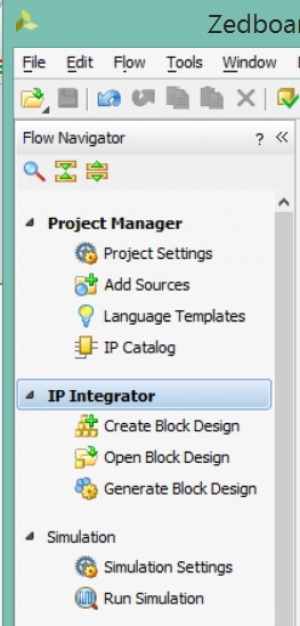
\includegraphics[width=0.2\textwidth]{images/image_7.jpg}
\end{figure}\\
Definiamo il nome e proseguiamo con la scelta dei componenti.\\
Cliccando il pulsante "Add IP" andiamo a cercare il processing system, che sarà obbligatoriamente \textbf{ZYNQ7 Processing System}.\\
Da questo punto possiamo aggiungere qualsiasi elemento di nostro interesse al fine di creare la struttura che più necessitiamo, effettuando ad ogni inserimento il comando \textit{Run Connection Automation} che ci sarà consigliato da Vivado.\\
Una volta inseriti tutti gli elementi richiesti procediamo con la rigenerazione del layout tramite il comando \verb|regenerate_bd_layout|.\\
Procediamo con le simulazioni e le sintesi al fine di poter generare il bitstream.
\subsubsection{Creazione HDL Wrapper}
L'HDL Wrapper è un file di High definition Level, che ci permette di definire il nostro progetto, tramite esso effettueremo le sintesi ed il bitstream.\\
Al fine di crearlo basterà cliccare con il tasto destro sul design creato in precedenza e cliccare la dicitura \textit{Create HDL Wrapper}
\begin{figure}[h]
\centering
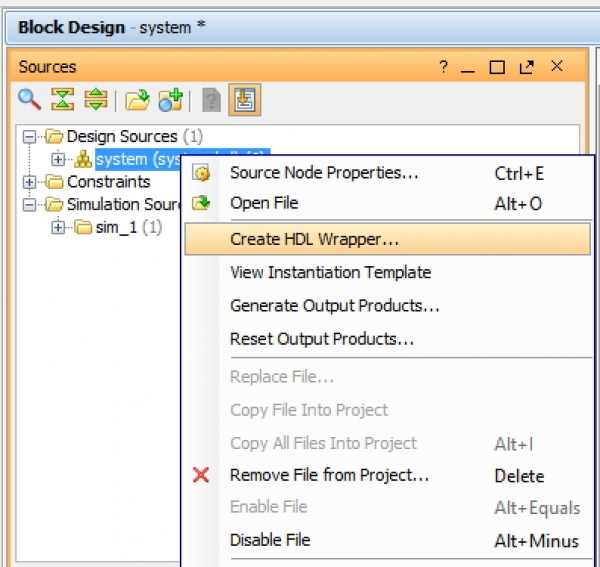
\includegraphics[width=0.4\textwidth]{images/image_20.jpg}
\end{figure}\\
\subsubsection{Sintesi}
Adesso dobbiamo avviare la sintesi, cosi da far tradurre il file HDL in una netlist\footnote{Contiene tutti i componenti che ci servono}, al fine di farla partire usiamo il pulsante \textit{Run Synthesis} che si trova nella tool bar di sinistra.
\subsubsection{Implementazione}
Questo processo mappa la sintesi che abbiamo svolto nel chip che abbiamo selezionato, nel nostro caso la zedboard. Anche qui troviamo la possibilità di far partire il tutto tramite il pulsante \textit{Run Implementation} nella tool bar di sinistra.
\subsection{Generazione del bistream}
Una volta terminati tutti questi passaggi andati a buon fine possiamo creare il file ".bit" che ci servirà più avanti per definire il kernel di petalinux. Al fine di far partire la generazione si usa il comando \textit{Generate Bitstream} presente nella tool bar di sinistra.
\subsection{Export del file di developing}\label{ExportVivado}
Al fine di creare sul nostro hardware l'immagine di petalinux, al fine di far ciò:
\begin{itemize}
\item Una volta seguiti tutti gli step precedenti clicco in alto a sinistra il pulsante file
\item Export, il terzultimo pulsante
\item Export hardware
\item Una volta aperta la finestra andiamo avanti e selezioniamo \textbf{Include bitstream}
\item Diamo un nome ed una directory ed abbiamo esportato tutto il necessario per petalinux
\end{itemize}


\chapter{}

\section{Programmazione StandAlone}
\label{Standalone}
Al fine di effettuare la programmazione StandAlone, basterà seguire i passaggi visti in precedenza fino al build del progetto, una volta che il progetto sarà buildato sarà necessario aver installati i driver della scheda.
\subsection{Installazione Driver}
Spostiamoci nella cartella d'installazione di vivado e dopodichè nel seguente path
\begin{lstlisting}
/data/xicom/cable_drivers/lin64/install_script/install_drivers/
\end{lstlisting}
da qui dovremmo semplicemente eseguire lo script.
\subsection{Flash}
Al fine di effettuare il flash sulla scheda dovremmo ritornare nel IDE, collegare la scheda nella micro USB J17, quella vicino i connettori audio, ed eseguire i seguenti passaggi:
\begin{itemize}
    \item Xilnix -> Program Device. In questa schermata che ci comparirà dobbiamo selezionare il bitstream collegato al nostro progetto e clicchiamo program.
    \item Una volta effettuato questo passaggio, clicchiamo sul progetto tasto destro \textit{Run As -> Launch Hardware}, dopodichè avremo sulla scheda ciò che abbiamo programmato.
\end{itemize}
\subsection{Collegamento Tramite UART}
Al fine di vedere il risultato a schermo della programmazione che si sta effettuando, bisogna connettersi tramite UART al connettore micro USB J14 e tramite un monitor seriale \href{https://ttssh2.osdn.jp/index.html.en}{Tera Term} su windows e tio su linux, connettersi alla scheda che solitamente sotto ambiente windows sarà COM* e sotto linux /dev/ttyACM* con un baudrate\footnote{velocità di trasmissione} di 115200, da qui potremmo interfacciarci con la scheda per usufruire del codice bare-metal che è stato caricato. \\
Questo metodo è equivalente se è presente petalinux sulla scheda.



\chapter{}

\section{Petalinux}
\label{petalinuxinst}
Per installare Petalinux, assicuriamoci che dopo l'installazione del pacchetto Vivado e Vitis restino al più 3GB.\\
Soddisfatto questo requisito, abbiamo la possibilità di percorrere due strade, l'installazione tramite self-extracting pack (una sorta di zip), ed l'installer della xilnix. Noi useremo il self-extracting pack, tanto sono equivalenti.\\
\subsection{Installazione}
Scarichiamo il file presente alla pagina \href{https://www.xilinx.com/support/download/index.html/content/xilinx/en/downloadNav/embedded-design-tools.html}{Petalinux}, se si usa una versione del sistema operativo compatibile anche l'ultima versione(2021.2) è funzionante, altrimenti usare la versione (2020.3).\\
\subsection{Requisiti}
Solitamente le dipendenze sono:
\begin{lstlisting}
sudo apt-get -y install iproute2 \
gcc \
g++ \
net-tools \
libncurses5-dev \
zlib1g:i386 \
libssl-dev \
flex \
bison \
libselinux1 \
xterm \
autoconf \
libtool \
texinfo \
zlib1g-dev \
gcc-multilib \
build-essential \
screen \
pax \
gawk \
python3 \
python3-pexpect \
python3-pip \
python3-git \
python3-jinja2 \
xz-utils \
debianutils \
iputils-ping \
libegl1-mesa \
libsdl1.2-dev \
pylint3 \
cpio
\end{lstlisting}
\subsection{Installazione}
\label{InstPeta}
Una volta scaricato il file assegnare ad esso i permessi d'esecuzione e spostarlo nella directory desiderata. Una volta effettuati questi passaggi eseguire il seguente comando:
\begin{lstlisting}
./petalinux-v<petalinux-version>-final-installer.run --dir /home/<user>/
petalinux/<petalinux-version>
\end{lstlisting}
Aggiungendo l'argomento 
\begin{lstlisting}
--platform "arm"
\end{lstlisting}
si può ridurre il peso dell'installazione a solo le zynq arm.\\
\subsection{Setup dell'ambiente lavorativo}
\label{SetupPeta}
Al fine di poter usare il tool bisogna eseguire il seguente comando:
\begin{lstlisting}
$ source <path-to-installed-PetaLinux>/settings.sh
$ source <path-to-installed-PetaLinux>/settings.csh
\end{lstlisting}
In base al tipo di Shell in cui ci troviamo.\\
Se l'output dovesse essere di questo tipo:
\begin{lstlisting}
PetaLinux environment set to '/opt/pkg/petalinux'
INFO: Checking free disk space
INFO: Checking installed tools
INFO: Checking installed development libraries
INFO: Checking network and other services
WARNING: No tftp server found - please refer to "UG1144 <petalinuxversion> PetaLinux Tools Documentation Reference Guide" for its impact
and solution
\end{lstlisting}
O al più presentare il seguente warning:
\begin{lstlisting}
WARNING: /bin/sh is not bash
\end{lstlisting}
Tutto è andato a buon fine e si può procedere con la creazione di una build.


\chapter{}
\section{Usare l'SD}
\label{sd}
\begin{itemize}
\item Formattare un SD da almeno 8GB, in due partizioni, la prima che useremo come BOOT in FAT32, con una dimensione di almeno 1GB, la seconda che useremo come root in ext4, da almeno 6GB.
\item Ora spostiamo i file :
\begin{itemize}
\item BOOT.BIN
\item image.ub, è l'immagine di linux
\item boot.scr
\end{itemize}
\item Estraiamo rootfs.tar.gz nella partizione di root
\item inseriamo l'sd nella scheda assicurandoci che sia impostata in boot da SD, quindi connettiamoci all'usb J14 e tramite un terminale seriale vediamo il boot della scheda.
\end{itemize}


\chapter{}
\section{Installazione BootGen}
\label{installazioneBoot}
Per installare bootgen è necessario usare il tool di download precedentemente scaricato in \ref{ExportVivado} e nel menu di selezione per l'installazione scegliere BOOTGEN.


\chapter{}
\section{Cross Compilazione}
\label{crossComp}
Per effettuare la cross-compilazione la strada più semplice è quella di sfruttare il cross compilatore già presente nella console di vivado, quindi per far ciò si avvii tramite shell vivado e ci si sposti nella cartella contentente il file in C, per compilare eseguire il seguente comando:
\begin{lstlisting}[language=sh, label=lst:sh, caption={Cross-compilazione}]
arm-linux-gnueabihf-gcc [nome].c -o [nome].out
\end{lstlisting}



\chapter{}
\section{Codice completo driver GPIO}
\label{GPIO}
\begin{lstlisting}[language=c, label=lst:sh, caption={Codice completo del driver GPIO}]

#include <unistd.h>
#include <time.h>
#include <stdio.h>
#include <stdlib.h>
#include <string.h>
#include <fcntl.h>
#include <sys/mman.h>
#include <sys/time.h>
#include <sys/types.h>
#include <sys/stat.h>

#define GPIO_BASE_ADDRESS       0x42000000
#define GPIO_MAP_SIZE           0x1000

#define XAXIGPIO_DATA_OFFSET    0x00000000

typedef unsigned long uint32;


int main(int argc, char *argv[]){
    unsigned long ii;
    int memfd;
    void *gpioMapAddr = NULL;

    if ( (memfd = open("/dev/mem", O_RDWR | O_DSYNC)) == -1 ){
        printf("Non riesco ad aprire /dev/mem.\n");
        exit(-1);
    }

    gpioMapAddr = mmap(0, GPIO_MAP_SIZE, PROT_READ | PROT_WRITE, MAP_SHARED, memfd, GPIO_BASE_ADDRESS);
    if (gpioMapAddr == (void *) -1){
        printf("Non posso mappare il CDMA.\n");
        exit(-1);
    }
    
    printf("GPIO mappato %p\n", gpioMapAddr);

    for(ii=0; ii<256; ii++){
        *((volatile unsigned long*) (gpioMapAddr + XAXIGPIO_DATA_OFFSET)) = ii;
        printf("led = 0x%02x\n", ii);
        usleep(20000); // sleep 20ms
    }
}

\end{lstlisting}
Qualora si volesse usare un GPIO dual channell, bisogna modificare l'offset che di default è 
$$GPIO\_BASE\_ADDRESS+ 0x08$$



\chapter{}
\section{Generazione automatica del file .bin}
\label{autoBOOT}
Al fine di effettuare la generazione automatica del file sarà necessario eseguire il seguente script, passandogli come parametri:
\begin{itemize}
    \item path/to/bitstream
    \item Architettura
    \item path/to/output
\end{itemize}
Inoltre sarà necessario creare un file \textit{template.bif} da posizionare nella stessa cartella d'esecuzione dello script
\begin{lstlisting}[language=sh, label=lst:sh, caption={Codice completo generazione automatica file BIN}]
#!/bin/bash
TMP_PATH=$(mktemp -d)
print_invalid_usage() {
	echo "Invalid usage."
	echo "Usage: generate <input_file_path> <output_directory_path>"
}
generate_bin() {
	BIT_PATH="$1"
	ARCH="$2"
	OUTPUT_PATH="$3"

	BIT_NAME=$(basename "$BIT_PATH")
	TMP_BIT_PATH="$TMP_PATH/$BIT_NAME"
	cp "$BIT_PATH" "$TMP_BIT_PATH"

	BIF_TEMPLATE_PATH="$template.bif"
	TMP_BIF_PATH="$TMP_PATH/bitstream.bif"
	sed -r "s|template.bit|$TMP_BIT_PATH|" "$BIF_TEMPLATE_PATH" > "$TMP_BIF_PATH"

	TMP_BIN_PATH="$TMP_BIT_PATH.bin"
	bootgen -image "$TMP_BIF_PATH" -arch "$ARCH" -process_bitstream bin
	if [[ $? -ne 0 ]]; then
		echo "Bin file generation failed."
		exit 1
	fi

	echo
	echo "Generating bin file..."
	BIN_PATH=$(realpath "$OUTPUT_PATH/fpga-$BIT_NAME.bin")
	cp "$TMP_BIN_PATH" "$BIN_PATH"
	echo "bin: $BIN_PATH"
}
	BIT_PATH="$1"
	ARCH="$2"
	OUTPUT_PATH="$3"

	if [[ "$BIT_PATH" = "" ]]; then
		print_invalid_usage
		exit 1
	fi

	if [[ "$OUTPUT_PATH" = "" ]]; then
		print_invalid_usage
		exit 1
	fi

	if [[ ! -f "$BIT_PATH" ]]; then
		echo "Invalid bit file path provided."
		echo "Make sure the path to the bit file is right."
		exit 1
	fi

	if [[ ! -d "$OUTPUT_PATH" ]]; then
		echo "Invalid output directory provided."
		echo "Make sure the path to the output directory is right."
		exit 1
	fi

	case "$ARCH" in	"zynq")		;;	*)
		echo "Invalid arch provided."
		exit 1
		;;
	esac

	generate_bin "$BIT_PATH" "$ARCH" "$OUTPUT_PATH"


echo
echo "Cleaning up..."
rm -rf "$TMP_PATH"

echo
echo "Finished."

\end{lstlisting}



\chapter{}
\section{Script riprogrammazione}
\label{Riprogrammazione}
Il seguente script necessita come parametri:
\begin{itemize}
    \item Il percorso fino al file binario
    \item il nome del file binario
\end{itemize}
\begin{lstlisting}[language=sh, label=lst:sh, caption={Codice completo riprogrammazione automatica FPGA}]
echo 0 > /sys/class/fpga_manager/fpga0/flags
mkdir -p /lib/firmware/
$path = $1
$nameBIN = $2
cd $path
cp $nameBIN /lib/firmware/
echo $nameBIN > /sys/class/fpga_manager/fpga0/firmware
\end{lstlisting}





%%%%%%%%%%%%%%%%%%%%%%%%%%%%%%%%%%%%%%%%%%%%%%%%%%%%%%%%%%%%%%%


% BIBLIOGRAFIA
\phantomsection
\addcontentsline{toc}{chapter}{\refname}
\nocite{*}
\printbibliography
% RINGRAZIAMENTI - PERSONALIZZARE
\ringraziamenti
\textit{Ai professori Francesco Longo e Giovanni Merilino}\\
Per il supporto datomi durante la scrittura della tesi e durante la mia carriera universitaria.\\\\\\
\textit{A SIC - Stretto in Carena}\\
Per avermi permesso di crescere sia come persona che come Ingegnere, rendendo il percorso unico.\\\\\\
\textit{Ai miei amici e colleghi}\\
Per l'aiuto, il supporto, le risate ed il tempo passato insieme in dipartimento e non.\\\\\\
\textit{A Silvia}\\
Per essermi stata affianco in questo percorso nonostante tutte le avversità del tragitto.\\\\\\
\textit{Alla mia famiglia}\\
Per il supporto in ogni mia decisione e per essere il paracadute in una vita in caduta libera.
\end{document}
